% Options for packages loaded elsewhere
\PassOptionsToPackage{unicode}{hyperref}
\PassOptionsToPackage{hyphens}{url}
\PassOptionsToPackage{dvipsnames,svgnames,x11names}{xcolor}
%
\documentclass[
  letterpaper,
  onepage,
  openany]{report}

\usepackage{amsmath,amssymb}
\usepackage{lmodern}
\usepackage{iftex}
\ifPDFTeX
  \usepackage[T1]{fontenc}
  \usepackage[utf8]{inputenc}
  \usepackage{textcomp} % provide euro and other symbols
\else % if luatex or xetex
  \usepackage{unicode-math}
  \defaultfontfeatures{Scale=MatchLowercase}
  \defaultfontfeatures[\rmfamily]{Ligatures=TeX,Scale=1}
\fi
% Use upquote if available, for straight quotes in verbatim environments
\IfFileExists{upquote.sty}{\usepackage{upquote}}{}
\IfFileExists{microtype.sty}{% use microtype if available
  \usepackage[]{microtype}
  \UseMicrotypeSet[protrusion]{basicmath} % disable protrusion for tt fonts
}{}
\makeatletter
\@ifundefined{KOMAClassName}{% if non-KOMA class
  \IfFileExists{parskip.sty}{%
    \usepackage{parskip}
  }{% else
    \setlength{\parindent}{0pt}
    \setlength{\parskip}{6pt plus 2pt minus 1pt}}
}{% if KOMA class
  \KOMAoptions{parskip=half}}
\makeatother
\usepackage{xcolor}
\usepackage[left=.75in,right=.75in,textwidth=4.5in,marginparsep=.25in,marginparwidth=2.25in]{geometry}
\setlength{\emergencystretch}{3em} % prevent overfull lines
\setcounter{secnumdepth}{5}
% Make \paragraph and \subparagraph free-standing
\ifx\paragraph\undefined\else
  \let\oldparagraph\paragraph
  \renewcommand{\paragraph}[1]{\oldparagraph{#1}\mbox{}}
\fi
\ifx\subparagraph\undefined\else
  \let\oldsubparagraph\subparagraph
  \renewcommand{\subparagraph}[1]{\oldsubparagraph{#1}\mbox{}}
\fi

\usepackage{color}
\usepackage{fancyvrb}
\newcommand{\VerbBar}{|}
\newcommand{\VERB}{\Verb[commandchars=\\\{\}]}
\DefineVerbatimEnvironment{Highlighting}{Verbatim}{commandchars=\\\{\}}
% Add ',fontsize=\small' for more characters per line
\usepackage{framed}
\definecolor{shadecolor}{RGB}{241,243,245}
\newenvironment{Shaded}{\begin{snugshade}}{\end{snugshade}}
\newcommand{\AlertTok}[1]{\textcolor[rgb]{0.68,0.00,0.00}{#1}}
\newcommand{\AnnotationTok}[1]{\textcolor[rgb]{0.37,0.37,0.37}{#1}}
\newcommand{\AttributeTok}[1]{\textcolor[rgb]{0.40,0.45,0.13}{#1}}
\newcommand{\BaseNTok}[1]{\textcolor[rgb]{0.68,0.00,0.00}{#1}}
\newcommand{\BuiltInTok}[1]{\textcolor[rgb]{0.00,0.23,0.31}{#1}}
\newcommand{\CharTok}[1]{\textcolor[rgb]{0.13,0.47,0.30}{#1}}
\newcommand{\CommentTok}[1]{\textcolor[rgb]{0.37,0.37,0.37}{#1}}
\newcommand{\CommentVarTok}[1]{\textcolor[rgb]{0.37,0.37,0.37}{\textit{#1}}}
\newcommand{\ConstantTok}[1]{\textcolor[rgb]{0.56,0.35,0.01}{#1}}
\newcommand{\ControlFlowTok}[1]{\textcolor[rgb]{0.00,0.23,0.31}{#1}}
\newcommand{\DataTypeTok}[1]{\textcolor[rgb]{0.68,0.00,0.00}{#1}}
\newcommand{\DecValTok}[1]{\textcolor[rgb]{0.68,0.00,0.00}{#1}}
\newcommand{\DocumentationTok}[1]{\textcolor[rgb]{0.37,0.37,0.37}{\textit{#1}}}
\newcommand{\ErrorTok}[1]{\textcolor[rgb]{0.68,0.00,0.00}{#1}}
\newcommand{\ExtensionTok}[1]{\textcolor[rgb]{0.00,0.23,0.31}{#1}}
\newcommand{\FloatTok}[1]{\textcolor[rgb]{0.68,0.00,0.00}{#1}}
\newcommand{\FunctionTok}[1]{\textcolor[rgb]{0.28,0.35,0.67}{#1}}
\newcommand{\ImportTok}[1]{\textcolor[rgb]{0.00,0.46,0.62}{#1}}
\newcommand{\InformationTok}[1]{\textcolor[rgb]{0.37,0.37,0.37}{#1}}
\newcommand{\KeywordTok}[1]{\textcolor[rgb]{0.00,0.23,0.31}{#1}}
\newcommand{\NormalTok}[1]{\textcolor[rgb]{0.00,0.23,0.31}{#1}}
\newcommand{\OperatorTok}[1]{\textcolor[rgb]{0.37,0.37,0.37}{#1}}
\newcommand{\OtherTok}[1]{\textcolor[rgb]{0.00,0.23,0.31}{#1}}
\newcommand{\PreprocessorTok}[1]{\textcolor[rgb]{0.68,0.00,0.00}{#1}}
\newcommand{\RegionMarkerTok}[1]{\textcolor[rgb]{0.00,0.23,0.31}{#1}}
\newcommand{\SpecialCharTok}[1]{\textcolor[rgb]{0.37,0.37,0.37}{#1}}
\newcommand{\SpecialStringTok}[1]{\textcolor[rgb]{0.13,0.47,0.30}{#1}}
\newcommand{\StringTok}[1]{\textcolor[rgb]{0.13,0.47,0.30}{#1}}
\newcommand{\VariableTok}[1]{\textcolor[rgb]{0.07,0.07,0.07}{#1}}
\newcommand{\VerbatimStringTok}[1]{\textcolor[rgb]{0.13,0.47,0.30}{#1}}
\newcommand{\WarningTok}[1]{\textcolor[rgb]{0.37,0.37,0.37}{\textit{#1}}}

\providecommand{\tightlist}{%
  \setlength{\itemsep}{0pt}\setlength{\parskip}{0pt}}\usepackage{longtable,booktabs,array}
\usepackage{calc} % for calculating minipage widths
% Correct order of tables after \paragraph or \subparagraph
\usepackage{etoolbox}
\makeatletter
\patchcmd\longtable{\par}{\if@noskipsec\mbox{}\fi\par}{}{}
\makeatother
% Allow footnotes in longtable head/foot
\IfFileExists{footnotehyper.sty}{\usepackage{footnotehyper}}{\usepackage{footnote}}
\makesavenoteenv{longtable}
\usepackage{graphicx}
\makeatletter
\def\maxwidth{\ifdim\Gin@nat@width>\linewidth\linewidth\else\Gin@nat@width\fi}
\def\maxheight{\ifdim\Gin@nat@height>\textheight\textheight\else\Gin@nat@height\fi}
\makeatother
% Scale images if necessary, so that they will not overflow the page
% margins by default, and it is still possible to overwrite the defaults
% using explicit options in \includegraphics[width, height, ...]{}
\setkeys{Gin}{width=\maxwidth,height=\maxheight,keepaspectratio}
% Set default figure placement to htbp
\makeatletter
\def\fps@figure{htbp}
\makeatother
\newlength{\cslhangindent}
\setlength{\cslhangindent}{1.5em}
\newlength{\csllabelwidth}
\setlength{\csllabelwidth}{3em}
\newlength{\cslentryspacingunit} % times entry-spacing
\setlength{\cslentryspacingunit}{\parskip}
\newenvironment{CSLReferences}[2] % #1 hanging-ident, #2 entry spacing
 {% don't indent paragraphs
  \setlength{\parindent}{0pt}
  % turn on hanging indent if param 1 is 1
  \ifodd #1
  \let\oldpar\par
  \def\par{\hangindent=\cslhangindent\oldpar}
  \fi
  % set entry spacing
  \setlength{\parskip}{#2\cslentryspacingunit}
 }%
 {}
\usepackage{calc}
\newcommand{\CSLBlock}[1]{#1\hfill\break}
\newcommand{\CSLLeftMargin}[1]{\parbox[t]{\csllabelwidth}{#1}}
\newcommand{\CSLRightInline}[1]{\parbox[t]{\linewidth - \csllabelwidth}{#1}\break}
\newcommand{\CSLIndent}[1]{\hspace{\cslhangindent}#1}

\newcommand*{\plogo}{\fbox{$\mathcal{PL}$}} % Generic dummy publisher logo

\usepackage[utf8]{inputenc} %Required for inputting international characters
\usepackage[T1]{fontenc} %Output font encoding for international characters
%\usepackage[spanish]{babel}






\usepackage{booktabs}
\usepackage{longtable}
\usepackage{array}
\usepackage{multirow}
\usepackage{wrapfig}
\usepackage{float}
\usepackage{colortbl}
\usepackage{pdflscape}
\usepackage{tabu}
\usepackage{threeparttable}
\usepackage{threeparttablex}
\usepackage[normalem]{ulem}
\usepackage{makecell}
\usepackage{xcolor}
\makeatletter
\makeatother
\makeatletter
\@ifpackageloaded{bookmark}{}{\usepackage{bookmark}}
\makeatother
\makeatletter
\@ifpackageloaded{caption}{}{\usepackage{caption}}
\AtBeginDocument{%
\ifdefined\contentsname
  \renewcommand*\contentsname{Indice de contenidos}
\else
  \newcommand\contentsname{Indice de contenidos}
\fi
\ifdefined\listfigurename
  \renewcommand*\listfigurename{Listado de Figuras}
\else
  \newcommand\listfigurename{Listado de Figuras}
\fi
\ifdefined\listtablename
  \renewcommand*\listtablename{Listado de Tablas}
\else
  \newcommand\listtablename{Listado de Tablas}
\fi
\ifdefined\figurename
  \renewcommand*\figurename{Figura}
\else
  \newcommand\figurename{Figura}
\fi
\ifdefined\tablename
  \renewcommand*\tablename{Tabla}
\else
  \newcommand\tablename{Tabla}
\fi
}
\@ifpackageloaded{float}{}{\usepackage{float}}
\floatstyle{ruled}
\@ifundefined{c@chapter}{\newfloat{codelisting}{h}{lop}}{\newfloat{codelisting}{h}{lop}[chapter]}
\floatname{codelisting}{Listado}
\newcommand*\listoflistings{\listof{codelisting}{Listado de Listatdos}}
\makeatother
\makeatletter
\@ifpackageloaded{caption}{}{\usepackage{caption}}
\@ifpackageloaded{subcaption}{}{\usepackage{subcaption}}
\makeatother
\makeatletter
\@ifpackageloaded{tcolorbox}{}{\usepackage[many]{tcolorbox}}
\makeatother
\makeatletter
\@ifundefined{shadecolor}{\definecolor{shadecolor}{rgb}{.97, .97, .97}}
\makeatother
\makeatletter
\makeatother
\ifLuaTeX
\usepackage[bidi=basic]{babel}
\else
\usepackage[bidi=default]{babel}
\fi
\babelprovide[main,import]{spanish}
% get rid of language-specific shorthands (see #6817):
\let\LanguageShortHands\languageshorthands
\def\languageshorthands#1{}
\ifLuaTeX
  \usepackage{selnolig}  % disable illegal ligatures
\fi
\IfFileExists{bookmark.sty}{\usepackage{bookmark}}{\usepackage{hyperref}}
\IfFileExists{xurl.sty}{\usepackage{xurl}}{} % add URL line breaks if available
\urlstyle{same} % disable monospaced font for URLs
\hypersetup{
  pdftitle={Not used},
  pdfauthor={Not used},
  pdflang={es},
  colorlinks=true,
  linkcolor={blue},
  filecolor={Maroon},
  citecolor={Blue},
  urlcolor={Blue},
  pdfcreator={LaTeX via pandoc}}

\title{Not used}
\author{Not used}
\date{}

\begin{document}
  \begin{titlepage}
  %%%%%%%%%%%%%%%%%%%%%%%%%%%%%%%%%%%%%%%%%
  % Academic Title Page
  % LaTeX Template
  % Version 2.0 (17/7/17)
  %
  % This template was downloaded from:
  % http://www.LaTeXTemplates.com
  %
  % Original author:
  % WikiBooks (LaTeX - Title Creation) with modifications by:
  % Vel (vel@latextemplates.com)
  %
  % License:
  % CC BY-NC-SA 3.0 (http://creativecommons.org/licenses/by-nc-sa/3.0/)
  % 
  %%%%%%%%%%%%%%%%%%%%%%%%%%%%%%%%%%%%%%%%%


  	\newcommand{\HRule}{\rule{\linewidth}{0.5mm}} % Defines a new command for horizontal lines, change thickness here
  	
  	\center % Centre everything on the page
  	
  	%------------------------------------------------
  	%	Headings
  	%------------------------------------------------
  	
  	\textsc{\LARGE Universidad de Costa Rica}\\[1.5cm] % Main heading such as the name of your university/college
  	
  	\textsc{\Large Modelos Lineales}\\[0.5cm] % Major heading such as course name
  	
  %	\textsc{\large Minor Heading}\\[0.5cm] % Minor heading such as course title
  	
  	%------------------------------------------------
  	%	Title
  	%------------------------------------------------
  	
  	\HRule\\[0.4cm]
  	
  	{\huge\bfseries Pronóstico demográfico de\\ Costa Rica}\\[0.4cm] % Title of your document
  	
  	\HRule\\[1.5cm]
  	
  	%------------------------------------------------
  	%	Author(s)
  	%------------------------------------------------
  	
  	%\begin{minipage}{0.4\textwidth}
  	%	\begin{flushleft}
  	%		\large
  	%		\textit{Authores}\\
  	%		% B.J. \textsc{Blazkowicz}  Your name
  	%		David Zumbado \\
  	%		Ignacio Barrantes \\
  	%		Leonardo Blanco
  	%	\end{flushleft}
  	%\end{minipage}
  	%~
  	%\begin{minipage}{0.4\textwidth}
  	%	\begin{flushright}
  	%		\large
  	%		\textit{Profesor}\\
  	%		 %Dr. Caroline \textsc{Becker}  Supervisor's name
  	%	\end{flushright}
  	%\end{minipage}
  	
  	% If you don't want a supervisor, uncomment the two lines below and comment the code above
  	{\large\textit{Autores}}\\
  	David Zumbado \\ % Your name
  	Leonardo Blanco \\
  	Ignacio Barrantes
  	
  	%------------------------------------------------
  	%	Date
  	%------------------------------------------------
  	
  	\vfill\vfill\vfill % Position the date 3/4 down the remaining page
  	
  	{\large\today} % Date, change the \today to a set date if you want to be precise
  	
  	%------------------------------------------------
  	%	Logo
  	%------------------------------------------------
  	
  	%\vfill\vfill
  	%\includegraphics[width=0.2\textwidth]{placeholder.jpg}\\[1cm] % Include a department/university logo - this will require the graphicx package
  	 
  	%----------------------------------------------------------------------------------------
  	
  	\vfill % Push the date up 1/4 of the remaining page
  	
  	  
  \end{titlepage}

  \ifdefined\Shaded\renewenvironment{Shaded}{\begin{tcolorbox}[borderline west={3pt}{0pt}{shadecolor}, enhanced, boxrule=0pt, breakable, frame hidden, interior hidden, sharp corners]}{\end{tcolorbox}}\fi

\renewcommand*\contentsname{Indice de contenidos}
{
\hypersetup{linkcolor=}
\setcounter{tocdepth}{2}
\tableofcontents
}
\listoffigures
\listoftables
\bookmarksetup{startatroot}

\hypertarget{section}{%
\chapter*{}\label{section}}
\addcontentsline{toc}{chapter}{}

\bookmarksetup{startatroot}

\hypertarget{bituxe1cora-1}{%
\chapter{Bitácora 1}\label{bituxe1cora-1}}

En el proyecto se buscará realizar análisis demográfico, específicamente
se centrará en el pronóstico de la cantidad de defunciones en Costa
Rica.

\hypertarget{parte-1}{%
\section{Parte 1}\label{parte-1}}

\hypertarget{caracteruxedsticas-generales-de-la-tabla}{%
\subsection{Características generales de la
tabla}\label{caracteruxedsticas-generales-de-la-tabla}}

La tabla de datos proviene del Instituto Nacional de Estadística y
Censos (INEC) de Costa Rica y es de acceso público, descargable desde la
página web del instituto, como puede consultarse en INEC (2021). Esta
base presenta los principales indicadores demográficos anuales de Costa
Rica durante el periodo 1950-2020. Incluye en total 18 variables, entre
las cuales están el año, la población total al 30 de junio de cada año,
desagregado también por sexo, así como la cantidad de defunciones.

\hypertarget{variables-de-estudio}{%
\subsection{Variables de estudio}\label{variables-de-estudio}}

\textbf{Población de estudio:} La población de estudio son aquellas
personas que vivían en Costa Rica entre los años 1950-2020 y mueren en
este periodo.

\textbf{Muestra observada:} La muestra observada, son todas aquellas
personas que vivían en Costa Rica y al morir son registrados por el
Instituto Nacional de Estadística y Censo.

\textbf{Unidad estadística o individuos}: La unidad estadística es el
recuento anual de defunciones en Costa Rica.

\textbf{Variables de estudio:} Son un total de 18 variables, las cuales
según {«Indicadores demográficos 2019»} (2020) se tiene:

\textbf{Año:} Esta variable indica el año.

\textbf{Total:} Esta variable registra la población total.

\textbf{Hombres:} Esta variable registra la población total de hombres.

\textbf{Mujeres:} Esta variable se encarga de registar el total de
mujeres.

\textbf{Nacimientos:} Esta variable registra el total de nacimientos.

\textbf{Defunciones:} Esta variable registra el total de defunciones.

\textbf{Defunciones infantiles:} Esta variable registra las defunciones
de infantes (niños y niñas).

\textbf{Defunciones neonatales:} Esta variable registra las defunciones
de recién nacidos, hace referencia a la mortalidad de los nacidos antes
de alcanzar los 28 días de edad.

\textbf{Defunciones fetales:} Esta variable registra las defunciones de
fetos, se refiere a la mortalidad de un bebé antes o durante el parto.

\textbf{Tasa de crecimiento:} Esta variable registra la tasa de
crecimiento de la población costarricense.Se refiere al crecimiento de
la población entre dos fechas sin contemplar la migración.

\textbf{Tasa de natalidad:} Esta variable registra la tasa de
nacimientos registrados en la población costarricenses.

\textbf{Tasa de mortalidad:} Esta variable registra la tasa de muertes
en su totalidad.

\textbf{Tasa de mortalidad infantil} Esta variable registra la tasa de
muertes infantiles.

\textbf{Tasa de mortalidad neonatal:} Esta variable registra la tasa de
muertes neonatales.

\textbf{Tasa de mortalidad fetal:} En esta variable se registra la tasa
de muertes fetales.

\textbf{Tasa global de fecundidad:} Esta variable registra la tasa de
fecundidad global (TGF), la cual indica cantidad de hijos e hijas que en
promedio tendría cada mujer al final del periodo fértil, si durante su
vida tiene sus hijos e hijas de acuerdo a las tasas de fecundidad por
edad observadas en el país y año de interés y, además estas mujeres no
están afectadas por la mortalidad desde el nacimiento hasta el final de
periodo fértil.

\textbf{Tasa bruta de reproducción:} Esta variable hace referencia a el
cantidad de hijas que en promedio tendría cada mujer al final del
periodo fértil, si durante su vida tiene sus hijos e hijas de acuerdo a
las tasas de fecundidad por edad observadas en el país y año de interés
y, además estas mujeres no están afectadas por la mortalidad desde el
nacimiento hasta el final de periodo fértil.

\textbf{Tasa neta de reproducción:} es el número de hijas que en
promedio tendría cada mujer al final del periodo fértil, si durante su
vida tiene sus hijos e hijas de acuerdo a las tasas de fecundidad por
edad observadas en el país y año de interés y, además estas mujeres sí
están afectadas por la mortalidad por edad observada en el país y año de
interés desde el nacimiento hasta el final de periodo fértil.

\hypertarget{clasificaciuxf3n-de-las-variables}{%
\subsection{Clasificación de las
variables}\label{clasificaciuxf3n-de-las-variables}}

Todas las variables de la tabla utilizada son numéricas donde cinco
identifican cantidades absolutas registradas con respecto a la cantidad
de nacimientos, defunciones, etc, y nueve variables son tasas de
variabilidad con respecto al año anterior, o como un porcentaje de la
población.

\hypertarget{parte-2}{%
\section{Parte 2}\label{parte-2}}

\hypertarget{pregunta-central-de-investigaciuxf3n}{%
\subsection{Pregunta central de
investigación}\label{pregunta-central-de-investigaciuxf3n}}

La pregunta formulada es: ¿Cómo se puede realizar un pronóstico de la
serie de defunciones totales anuales de Costa Rica?

\hypertarget{objeto-de-la-investigaciuxf3n}{%
\subsection{Objeto de la
investigación}\label{objeto-de-la-investigaciuxf3n}}

La cantidad de defunciones totales anuales ocurridas en Costa Rica y
registradas por el Instituto Nacional de Estadística y Censos del año
1950 hasta el año 2020.

\hypertarget{conceptos-delimitadores-de-la-pregunta-de-investigaciuxf3n}{%
\subsection{Conceptos delimitadores de la pregunta de
investigación}\label{conceptos-delimitadores-de-la-pregunta-de-investigaciuxf3n}}

\begin{itemize}
\item
  Defunciones totales anuales: Según Macció, Centro Latinoamericano de
  Demografia, et~al. (1985), la mortalidad o defunción se emplea para
  expresar la acción de la muerte sobre la población. Esta se mide en
  valores absolutos y sobre el año calendario.
\item
  Pronóstico: Según Brownlee (2020) la realización de predicciones sobre
  el futuro se denomina extrapolación en el tratamiento estadístico
  clásico de los datos de las series temporales. Los campos más modernos
  que se centran en el tema, lo denominan pronóstico de series
  temporales.El pronóstico consiste en tomar modelos ajustados a datos
  históricos y utilizarlos para predecir observaciones futuras.
\item
  Serie: De acuerdo a Macció, Centro Latinoamericano de Demografia,
  et~al. (1985) una series cronológica o crónica se le llama a ``la que
  forman los valores sucesivos que una cierta variable ha tomado en el
  transcurso del tiempo''.
\end{itemize}

\hypertarget{principios}{%
\subsection{Principios}\label{principios}}

Rees (2020) afirma que una de las mayores contribuciones de la
demografía ha sido el desarrollo de modelos para la proyección de
futuras poblaciones, lo cuál está estrechamente relacionado con la
proyección de defunciones. De acuerdo al autor, dos de los modelos más
importantes y usados en Demografía cuando a proyección poblacional se
refiere, están el de Cohorte-Componente (\emph{The Cohort--Component
Model for Projecting the Population}) y el de Proyecciones
Probabilísticas (\emph{Probabilistic Projections}).

El modelo de Cohorte-Componente utiliza datos de nacimientos, muertes y
migración (a estos factores se les conoce como componentes de cambio) a
nivel de cohortes. De acuerdo al Diccionario Demográfico Multilingüe, un
cohorte es ``conjunto de individuos que han vivido un cierto
acontecimiento durante un mismo período'' (1985); y en el marco del
modelo puede referirse a grupos de edad. Usualmente, los cohortes están
desagregados por sexo (Wilson y Rees 2021).

Por otro lado, el modelo de Proyecciones Probabilísticas, el cual
también es establecido en Rees (2020) trata de estimar la población
futura a través de los distribuciones de error de ciertos componentes
como la tasa de fertilidad. Con estas se pueden proyectar año a año y
bajo la combinación de cientos de estos componentes se puede construir
escenarios posibles. Cada una de estas distribuciones se puede derivar
utilizando datos históricos y a través del uso de modelos de series de
tiempo auto-regresivas, o de censos o opiniones experta. Bajo este
enfoque se construyen varios escenarios alrededor de una mediana y que
se dispersan producto de las distribuciones de incertidumbre pero que al
final logran construir un análogo del intervalo de confianza.

\bookmarksetup{startatroot}

\hypertarget{bitacora-2}{%
\chapter{Bitacora 2}\label{bitacora-2}}

\renewcommand\tablename{Tabla}

\hypertarget{punto-1}{%
\section{Punto 1}\label{punto-1}}

En la Tabla~\ref{tbl-tidy1} y Tabla~\ref{tbl-tidy2} se presentan las
primeras cinco líneas de la tabla de datos para las columnas 1 a 9 y 10
a 18 respectivamente. En conformidad con Wickham y Grolemund (2016), una
tabla en formato \emph{tidy} cumple que:

\begin{itemize}
\item
  Cada variable possee su propia columna
\item
  Cada observación posee su propia fila
\item
  Cada valor posee su propia celda
\end{itemize}

Se puede apreciar en las dos tablas mencionadas que la tabla de datos
cumple con el formato \emph{tidy}, pues las variables están dispuestas a
lo largo de las columnas y las observaciones a lo largo de las filas.

\hypertarget{tbl-tidy1}{}
\begin{landscape}\begin{table}
\caption{\label{tbl-tidy1}Primeras cinco filas y nueve columnas de la tabla de datos }\tabularnewline

\centering
\resizebox{\linewidth}{!}{
\begin{tabular}[t]{>{\raggedleft\arraybackslash}p{3cm}>{\raggedleft\arraybackslash}p{3cm}>{\raggedleft\arraybackslash}p{3cm}>{\raggedleft\arraybackslash}p{3cm}>{\raggedleft\arraybackslash}p{3cm}>{\raggedleft\arraybackslash}p{3cm}>{\raggedleft\arraybackslash}p{3cm}>{\raggedleft\arraybackslash}p{3cm}>{\raggedleft\arraybackslash}p{3cm}}
\toprule
\textbf{Año} & \textbf{Población total} & \textbf{Población de hombres} & \textbf{Población de mujeres} & \textbf{Nacimientos} & \textbf{Defunciones} & \textbf{Defunciones infantiles} & \textbf{Defunciones neonatales} & \textbf{Defunciones fetales}\\
\midrule
\cellcolor{gray!6}{1 950} & \cellcolor{gray!6}{868 934} & \cellcolor{gray!6}{438 185} & \cellcolor{gray!6}{430 749} & \cellcolor{gray!6}{37 248} & \cellcolor{gray!6}{9 769} & \cellcolor{gray!6}{3 358} & \cellcolor{gray!6}{974} & \cellcolor{gray!6}{1 103}\\
1 951 & 897 630 & 452 702 & 444 928 & 39 239 & 9 631 & 3 467 & 953 & 1 062\\
\cellcolor{gray!6}{1 952} & \cellcolor{gray!6}{929 173} & \cellcolor{gray!6}{468 613} & \cellcolor{gray!6}{460 560} & \cellcolor{gray!6}{42 461} & \cellcolor{gray!6}{9 902} & \cellcolor{gray!6}{3 811} & \cellcolor{gray!6}{1 083} & \cellcolor{gray!6}{1 012}\\
1 953 & 962 485 & 485 464 & 477 021 & 42 817 & 10 312 & 4 017 & 1 161 & 1 021\\
\cellcolor{gray!6}{1 954} & \cellcolor{gray!6}{997 535} & \cellcolor{gray!6}{503 219} & \cellcolor{gray!6}{494 316} & \cellcolor{gray!6}{48 157} & \cellcolor{gray!6}{9 713} & \cellcolor{gray!6}{3 856} & \cellcolor{gray!6}{1 210} & \cellcolor{gray!6}{1 135}\\
\addlinespace
1 955 & 1 035 424 & 522 378 & 513 046 & 48 903 & 9 998 & 4 065 & 1 233 & 1 095\\
\bottomrule
\multicolumn{9}{l}{\rule{0pt}{1em}\textit{Nota}}\\
\multicolumn{9}{l}{\rule{0pt}{1em}El conteo de población se realiza al 30 de junio de cada año.}\\
\end{tabular}}
\end{table}
\end{landscape}

\hypertarget{tbl-tidy2}{}
\begin{landscape}\begin{table}
\caption{\label{tbl-tidy2}Primeras cinco filas y segundas nueve columnas de la tabla de datos }\tabularnewline

\centering
\resizebox{\linewidth}{!}{
\begin{tabular}[t]{>{\raggedleft\arraybackslash}p{3cm}>{\raggedleft\arraybackslash}p{3cm}>{\raggedleft\arraybackslash}p{3cm}>{\raggedleft\arraybackslash}p{3cm}>{\raggedleft\arraybackslash}p{3cm}>{\raggedleft\arraybackslash}p{3cm}>{\raggedleft\arraybackslash}p{3cm}>{\raggedleft\arraybackslash}p{3cm}>{\raggedleft\arraybackslash}p{3cm}}
\toprule
\textbf{Tasa de crecimiento} & \textbf{Tasa de natalidad} & \textbf{Tasa de mortalidad} & \textbf{Tasa de mortalidad infantil} & \textbf{Tasa de mortalidad neonatal} & \textbf{Tasa de mortalidad fetal} & \textbf{Tasa global de fecundidad} & \textbf{Tasa bruta de reproducción} & \textbf{Tasa neta de reproducción}\\
\midrule
\cellcolor{gray!6}{31.62381} & \cellcolor{gray!6}{42.86632} & \cellcolor{gray!6}{11.242511} & \cellcolor{gray!6}{90.15249} & \cellcolor{gray!6}{26.14906} & \cellcolor{gray!6}{29.61233} & \cellcolor{gray!6}{-} & \cellcolor{gray!6}{-} & \cellcolor{gray!6}{-}\\
32.98464 & 43.71400 & 10.729365 & 88.35597 & 24.28706 & 27.06491 & - & - & -\\
\cellcolor{gray!6}{35.04084} & \cellcolor{gray!6}{45.69763} & \cellcolor{gray!6}{10.656788} & \cellcolor{gray!6}{89.75295} & \cellcolor{gray!6}{25.50576} & \cellcolor{gray!6}{23.83364} & \cellcolor{gray!6}{-} & \cellcolor{gray!6}{-} & \cellcolor{gray!6}{-}\\
33.77195 & 44.48589 & 10.713933 & 93.81788 & 27.11540 & 23.84567 & - & - & -\\
\cellcolor{gray!6}{38.53900} & \cellcolor{gray!6}{48.27600} & \cellcolor{gray!6}{9.737002} & \cellcolor{gray!6}{80.07143} & \cellcolor{gray!6}{25.12615} & \cellcolor{gray!6}{23.56874} & \cellcolor{gray!6}{-} & \cellcolor{gray!6}{-} & \cellcolor{gray!6}{-}\\
\addlinespace
37.57398 & 47.22993 & 9.655948 & 83.12373 & 25.21318 & 22.39126 & 6.96 & - & -\\
\bottomrule
\multicolumn{9}{l}{\rule{0pt}{1em}\textit{Nota}}\\
\multicolumn{9}{l}{\rule{0pt}{1em}El conteo de población se realiza al 30 de junio de cada año.}\\
\end{tabular}}
\end{table}
\end{landscape}

\hypertarget{parte-2-1}{%
\section{Parte 2}\label{parte-2-1}}

\hypertarget{resumen-de-cinco-nuxfameros}{%
\subsection{Resumen de cinco
números}\label{resumen-de-cinco-nuxfameros}}

En la tabla Tabla~\ref{tbl-resumen5numeros} se detalla el resumen de
cinco números para algunas variables relevantes de la tabla de datos.

\hypertarget{tbl-resumen5numeros}{}
\begin{table}
\caption{\label{tbl-resumen5numeros}Resumen de cinco números para algunas variables de la tabla de datos }\tabularnewline

\centering
\resizebox{\linewidth}{!}{
\begin{tabular}[t]{>{\raggedright\arraybackslash}p{3cm}>{\raggedleft\arraybackslash}p{3cm}>{\raggedleft\arraybackslash}p{3cm}>{\raggedleft\arraybackslash}p{3cm}>{\raggedleft\arraybackslash}p{3cm}>{\raggedleft\arraybackslash}p{3cm}>{\raggedleft\arraybackslash}p{3cm}>{\raggedleft\arraybackslash}p{3cm}>{\raggedleft\arraybackslash}p{3cm}}
\toprule
\textbf{ } & \textbf{Población total} & \textbf{Población de hombres} & \textbf{Población de mujeres} & \textbf{Nacimientos} & \textbf{Defunciones} & \textbf{Defunciones infantiles} & \textbf{Defunciones neonatales} & \textbf{Defunciones fetales}\\
\midrule
\cellcolor{gray!6}{\textbf{Mínimo}} & \cellcolor{gray!6}{868 934} & \cellcolor{gray!6}{438 185} & \cellcolor{gray!6}{430 749.0} & \cellcolor{gray!6}{37 248} & \cellcolor{gray!6}{8 596.0} & \cellcolor{gray!6}{462.0} & \cellcolor{gray!6}{344.0} & \cellcolor{gray!6}{329}\\
\textbf{Primer cuartil} & 1 638 283 & 827 590 & 810 692.5 & 59 589 & 9 897.5 & 765.0 & 537.0 & 526\\
\cellcolor{gray!6}{\textbf{Mediana}} & \cellcolor{gray!6}{2 646 142} & \cellcolor{gray!6}{1 339 573} & \cellcolor{gray!6}{1 306 569.0} & \cellcolor{gray!6}{70 004} & \cellcolor{gray!6}{11 376.0} & \cellcolor{gray!6}{1 345.0} & \cellcolor{gray!6}{807.0} & \cellcolor{gray!6}{691}\\
\textbf{Tercer cuartil} & 4 054 418 & 2 053 052 & 2 001 366.5 & 75 794 & 15 704.5 & 3 543.5 & 1 173.5 & 959\\
\cellcolor{gray!6}{\textbf{Máximo}} & \cellcolor{gray!6}{5 111 238} & \cellcolor{gray!6}{2 575 550} & \cellcolor{gray!6}{2 535 688.0} & \cellcolor{gray!6}{84 337} & \cellcolor{gray!6}{26 209.0} & \cellcolor{gray!6}{4 889.0} & \cellcolor{gray!6}{1 688.0} & \cellcolor{gray!6}{1 261}\\
\bottomrule
\end{tabular}}
\end{table}

\hypertarget{medidas-de-dispersiuxf3n}{%
\subsection{Medidas de dispersión}\label{medidas-de-dispersiuxf3n}}

En la tabla Tabla~\ref{tbl-estadisticos_dispersion} se detallan los
estadísticos de desviación estándar y rango intercuartílico para algunas
variables relevante de la tabla de datos.

\hypertarget{tbl-estadisticos_dispersion}{}
\begin{table}
\caption{\label{tbl-estadisticos_dispersion}Estadísticos de dispersión para algunas variables de la tabla de datos }\tabularnewline

\centering
\resizebox{\linewidth}{!}{
\begin{tabular}[t]{>{\raggedright\arraybackslash}p{3cm}>{\raggedleft\arraybackslash}p{3cm}>{\raggedleft\arraybackslash}p{3cm}>{\raggedleft\arraybackslash}p{3cm}>{\raggedleft\arraybackslash}p{3cm}>{\raggedleft\arraybackslash}p{3cm}>{\raggedleft\arraybackslash}p{3cm}>{\raggedleft\arraybackslash}p{3cm}>{\raggedleft\arraybackslash}p{3cm}}
\toprule
\textbf{ } & \textbf{Población total} & \textbf{Población de hombres} & \textbf{Población de mujeres} & \textbf{Nacimientos} & \textbf{Defunciones} & \textbf{Defunciones infantiles} & \textbf{Defunciones neonatales} & \textbf{Defunciones fetales}\\
\midrule
\cellcolor{gray!6}{\textbf{Desviación estándar}} & \cellcolor{gray!6}{1 340 677} & \cellcolor{gray!6}{677 255.2} & \cellcolor{gray!6}{663 434.1} & \cellcolor{gray!6}{11 274.6} & \cellcolor{gray!6}{4 428.495} & \cellcolor{gray!6}{1 396.199} & \cellcolor{gray!6}{366.604} & \cellcolor{gray!6}{241.5763}\\
\textbf{Rango intercuartílico} & 2 416 136 & 1 225 461.5 & 1 190 674.0 & 16 205.0 & 5 807.000 & 2 778.500 & 636.500 & 433.0000\\
\bottomrule
\end{tabular}}
\end{table}

Se observa que la variable población de hombres presenta mayor
dispersión respecto población de mujeres, esta mayor variabilidad en la
población de hombres se puede deber a diversos factores, entre ellos :
una diferencia en el número de defunciones, nacimientos, o número de
migrantes en la población masculina en relación con la de población
femenina.

Una observación importante, es que los nacimientos presentan una mayor
dispersión respecto a el número de defunciones. Es decir, se observa que
el número defunciones anuales presenta menor desviación respecto a la
media (desviación estándar) y una menor diferencia entre tercer cuartil
y primer cuartil de defunciones (IQR).

Análogamente, se observa que para los tipos de defunción: infantil,
neonatales y fetales. Se evidencia una mayor dispersión para las
defunciones infantiles, seguidas de las neonatales y por último, con
menor dispersión las defunciones fetales.

Finalmente, se observa una diferencia significativa entre la medidas de
dispersión desviación estándar y rango intercuartílico (IQR), esto se
debe a la sensibilidad de la desviación estándar a valores extremos, es
decir es posible que existan valores extremos (muy alto o muy bajos
respecto a la media) y por esta razón ambas medidas difieran
considerablemente, sin embargo para este caso en particular el orden en
el grado de dispersión (observe que la dispersión disminuye al avanzar
en la tabla de izquierda a derecha) se mantiene para ambos medidas.

\newpage

\hypertarget{tablas-de-frecuencia}{%
\subsection{Tablas de frecuencia}\label{tablas-de-frecuencia}}

\hypertarget{tbl-freq1}{}
\begin{table}
\caption{\label{tbl-freq1}Frecuencia de defunciones, población y tasa de mortalidad }\tabularnewline

\centering
\resizebox{\linewidth}{!}{
\begin{tabular}[t]{cccccc}
\toprule
\textbf{Defunciones} & \textbf{Frec. de defunciones} & \textbf{Población total} & \textbf{Frec. de poblacion} & \textbf{Tasa de mortalidad} & \textbf{Frec. de tasa}\\
\midrule
\cellcolor{gray!6}{(8.58e+03,1.04e+04]} & \cellcolor{gray!6}{23} & \cellcolor{gray!6}{(8.65e+05,1.29e+06]} & \cellcolor{gray!6}{11} & \cellcolor{gray!6}{(3.72,4.41]} & \cellcolor{gray!6}{39}\\
(1.04e+04,1.21e+04] & 18 & (1.29e+06,1.72e+06] & 9 & (4.41,5.1] & 8\\
\cellcolor{gray!6}{(1.21e+04,1.39e+04]} & \cellcolor{gray!6}{4} & \cellcolor{gray!6}{(1.72e+06,2.14e+06]} & \cellcolor{gray!6}{8} & \cellcolor{gray!6}{(5.1,5.78]} & \cellcolor{gray!6}{1}\\
(1.39e+04,1.56e+04] & 8 & (2.14e+06,2.57e+06] & 6 & (5.78,6.46] & 3\\
\cellcolor{gray!6}{(1.56e+04,1.74e+04]} & \cellcolor{gray!6}{5} & \cellcolor{gray!6}{(2.57e+06,2.99e+06]} & \cellcolor{gray!6}{6} & \cellcolor{gray!6}{(6.46,7.14]} & \cellcolor{gray!6}{3}\\
\addlinespace
(1.74e+04,1.92e+04] & 4 & (2.99e+06,3.41e+06] & 5 & (7.14,7.83] & 3\\
\cellcolor{gray!6}{(1.92e+04,2.09e+04]} & \cellcolor{gray!6}{3} & \cellcolor{gray!6}{(3.41e+06,3.84e+06]} & \cellcolor{gray!6}{5} & \cellcolor{gray!6}{(7.83,8.51]} & \cellcolor{gray!6}{6}\\
(2.09e+04,2.27e+04] & 2 & (3.84e+06,4.26e+06] & 6 & (8.51,9.19] & 1\\
\cellcolor{gray!6}{(2.27e+04,2.44e+04]} & \cellcolor{gray!6}{3} & \cellcolor{gray!6}{(4.26e+06,4.69e+06]} & \cellcolor{gray!6}{7} & \cellcolor{gray!6}{(9.19,9.88]} & \cellcolor{gray!6}{3}\\
(2.44e+04,2.62e+04] & 1 & (4.69e+06,5.12e+06] & 8 & (10.6,11.3] & 4\\
\bottomrule
\end{tabular}}
\end{table}

De la Tabla~\ref{tbl-freq1} se observa que históricamente las
defunciones totales de la mayoría de los años cae dentro del primero y
segundo intervalo, con una distribución más uniforme dentro de los
intervalos más altos. Por su parte la tasa de mortalidad bruta, la cual
se aprecia en las columnas cinco y seis, se muestra que en la mayoría de
años la tasa se ha mantenido entre 3.72 y 4.41. Esto quiere decir que la
cantidad de defunciones relativo a la población ha sido más o menos
constante en la mayoría de años. Por su parte, la población total se ha
distribuido más uniformemente en todos los intervalos por lo que se
concluye que el crecimiento población se ha movido más rápido que las
defunciones.

\hypertarget{tbl-freq2}{}
\begin{table}
\caption{\label{tbl-freq2}Frecuencia de nacimientos y tasa de natalidad }\tabularnewline

\centering
\resizebox{\linewidth}{!}{
\begin{tabular}[t]{cccc}
\toprule
\textbf{Nacimientos} & \textbf{Frec. de nacimientos} & \textbf{Tasa de nacimientos} & \textbf{Frec. de tasa}\\
\midrule
\cellcolor{gray!6}{(3.72e+04,4.2e+04]} & \cellcolor{gray!6}{2} & \cellcolor{gray!6}{(11.3,15.4]} & \cellcolor{gray!6}{8}\\
(4.2e+04,4.67e+04] & 2 & (15.4,19.6] & 12\\
\cellcolor{gray!6}{(4.67e+04,5.14e+04]} & \cellcolor{gray!6}{2} & \cellcolor{gray!6}{(19.6,23.7]} & \cellcolor{gray!6}{6}\\
(5.14e+04,5.61e+04] & 4 & (23.7,27.8] & 5\\
\cellcolor{gray!6}{(5.61e+04,6.08e+04]} & \cellcolor{gray!6}{10} & \cellcolor{gray!6}{(27.8,31.9]} & \cellcolor{gray!6}{19}\\
\addlinespace
(6.08e+04,6.55e+04] & 7 & (31.9,36.1] & 3\\
\cellcolor{gray!6}{(6.55e+04,7.02e+04]} & \cellcolor{gray!6}{9} & \cellcolor{gray!6}{(36.1,40.2]} & \cellcolor{gray!6}{1}\\
(7.02e+04,7.49e+04] & 15 & (40.2,44.3] & 3\\
\cellcolor{gray!6}{(7.49e+04,7.96e+04]} & \cellcolor{gray!6}{9} & \cellcolor{gray!6}{(44.3,48.4]} & \cellcolor{gray!6}{11}\\
(7.96e+04,8.44e+04] & 11 & (48.4,52.6] & 3\\
\bottomrule
\end{tabular}}
\end{table}

En la tabla Tabla~\ref{tbl-freq2} se observa que los nacimientos en
nuestro país a lo largo de los años tiene una distribución más uniforme
para los últimos intervalos de la tabla.

Por otro lado, para el caso de la tasa de nacimientos se observa un
comportamiento menos uniforme a diferencia de los observado para la tasa
de mortalidad. En este caso, se observa que la frecuencia oscila entre
valores menores a 6 pero con ciertos repuntes altos de frecuencia para
ciertos intervalos por lo que la tasa de nacimientos no se mantiene en
cierto intervalo específico.

\hypertarget{parte-3-propuesta-de-uve}{%
\section{Parte 3: Propuesta de UVE}\label{parte-3-propuesta-de-uve}}

\begin{figure}[H]

{\centering 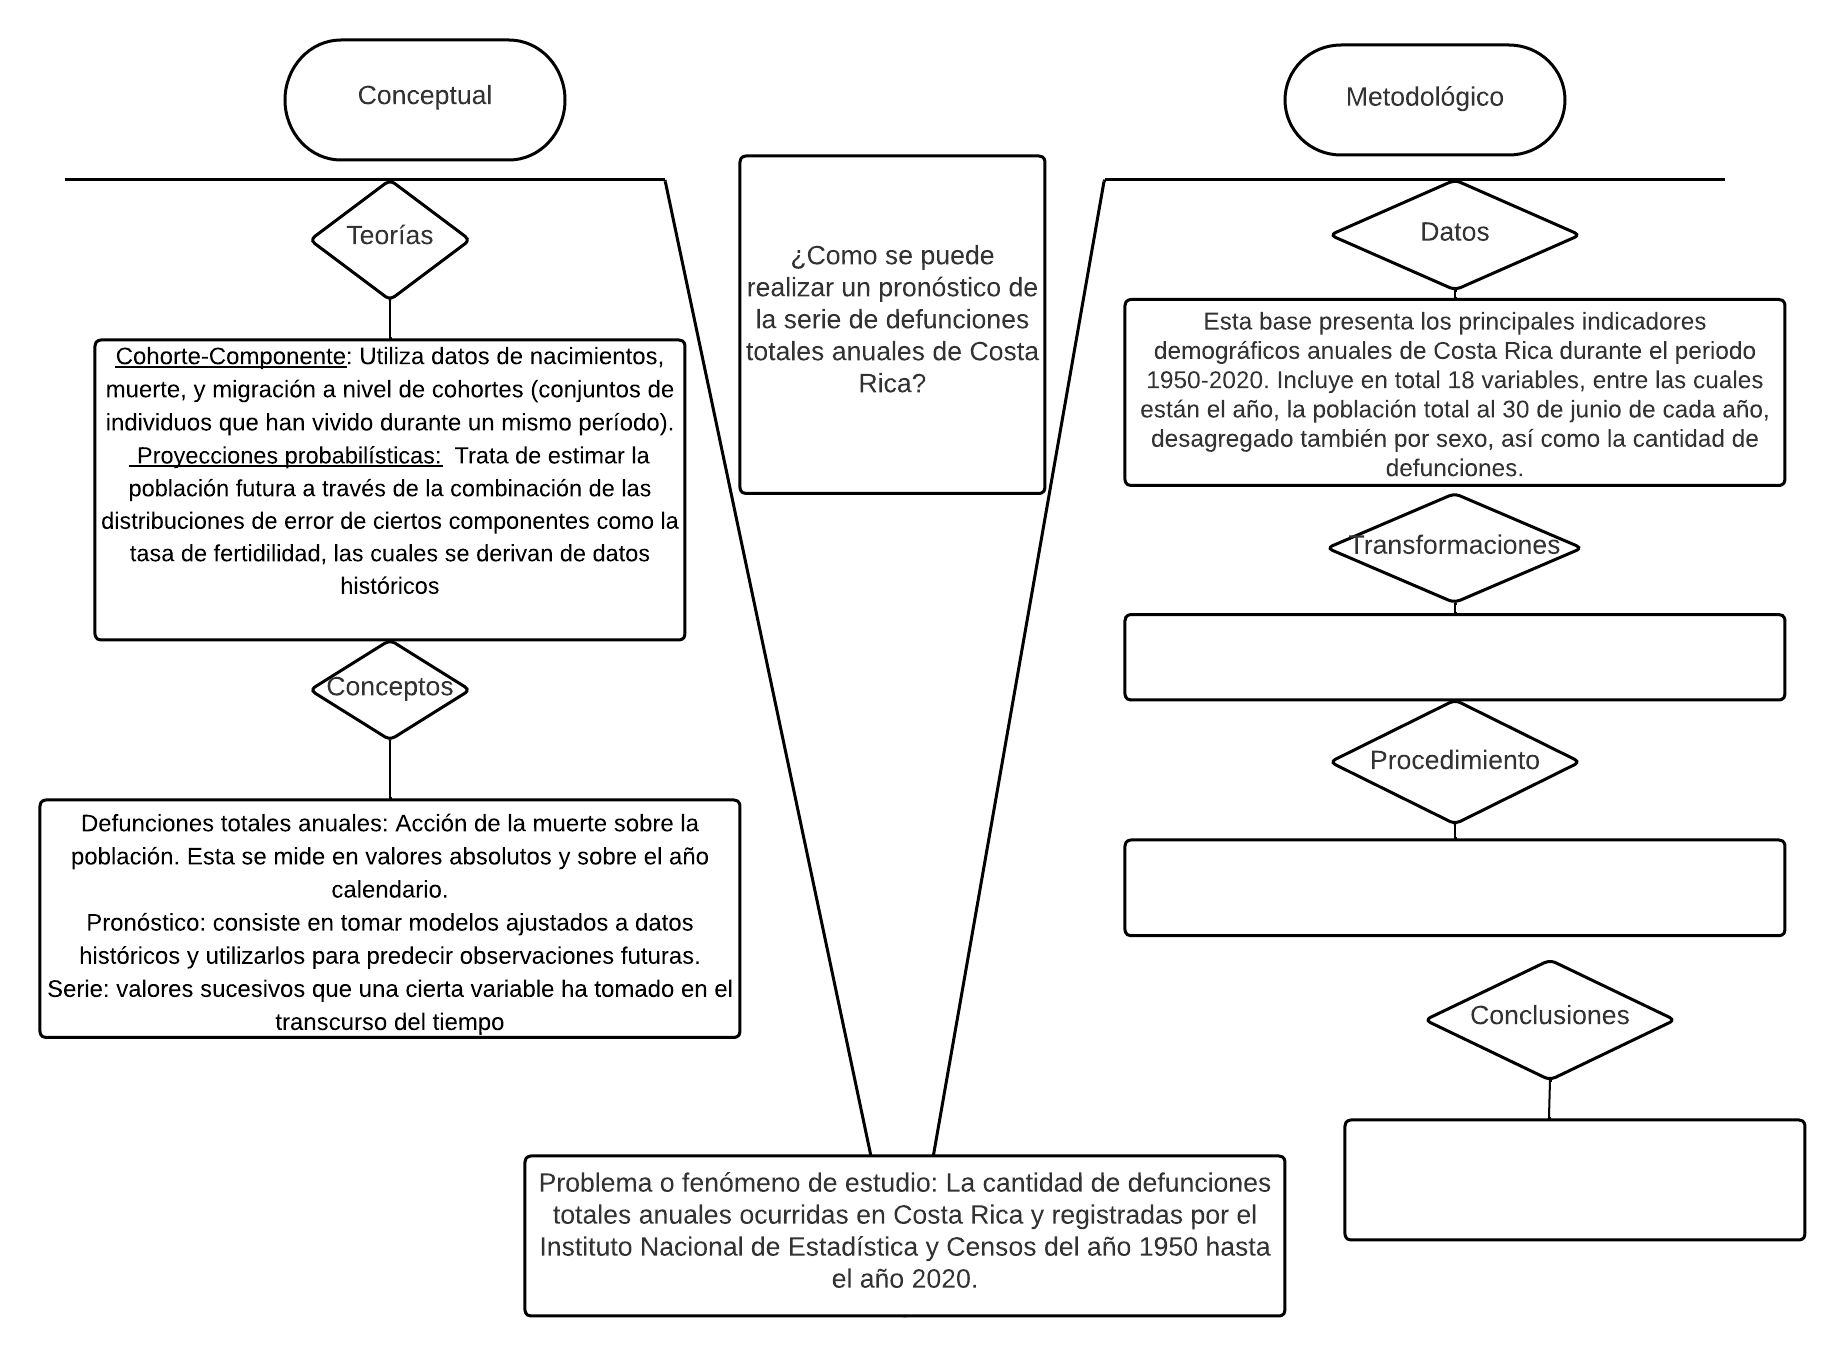
\includegraphics[width=6.25in,height=\textheight]{./Images/UVE Flecha.png}

}

\caption{Borrador de la UVE Heurística}

\end{figure}

\bookmarksetup{startatroot}

\hypertarget{bitacora-3}{%
\chapter{Bitacora 3}\label{bitacora-3}}

\hypertarget{distribuciuxf3n-de-la-variable-cuantitativa}{%
\section{Distribución de la variable
cuantitativa}\label{distribuciuxf3n-de-la-variable-cuantitativa}}

\begin{figure}[H]

{\centering \includegraphics{./Bit3_files/figure-pdf/fig-histdefunciones-1.pdf}

}

\caption{\label{fig-histdefunciones}Histograma de las defunciones
totales entre 1950 y 2020}

\end{figure}

La Figura~\ref{fig-histdefunciones} muestra la distribución de la
variable cuantitativa de defunciones totales anuales, la cual es de
principal interés en este trabajo. Se muestra poca simetría y una
acumulación muy marcada en los cantidades más pequeñas, lo que quiere
decir que la mayoría de años registrados presentaron defunciones totales
de menos de 1500 al año.

\hypertarget{asoaciaciuxf3n-de-variables}{%
\section{Asoaciación de variables}\label{asoaciaciuxf3n-de-variables}}

En la Figura~\ref{fig-defunciones_ano} se muestra la cantidad total de
defunciones para el periodo 1950-2020. Destaca una tendencia creciente
muy marcada a partir de cerca de 1980 y hasta el final del periodo
considerado.

\begin{figure}[H]

{\centering 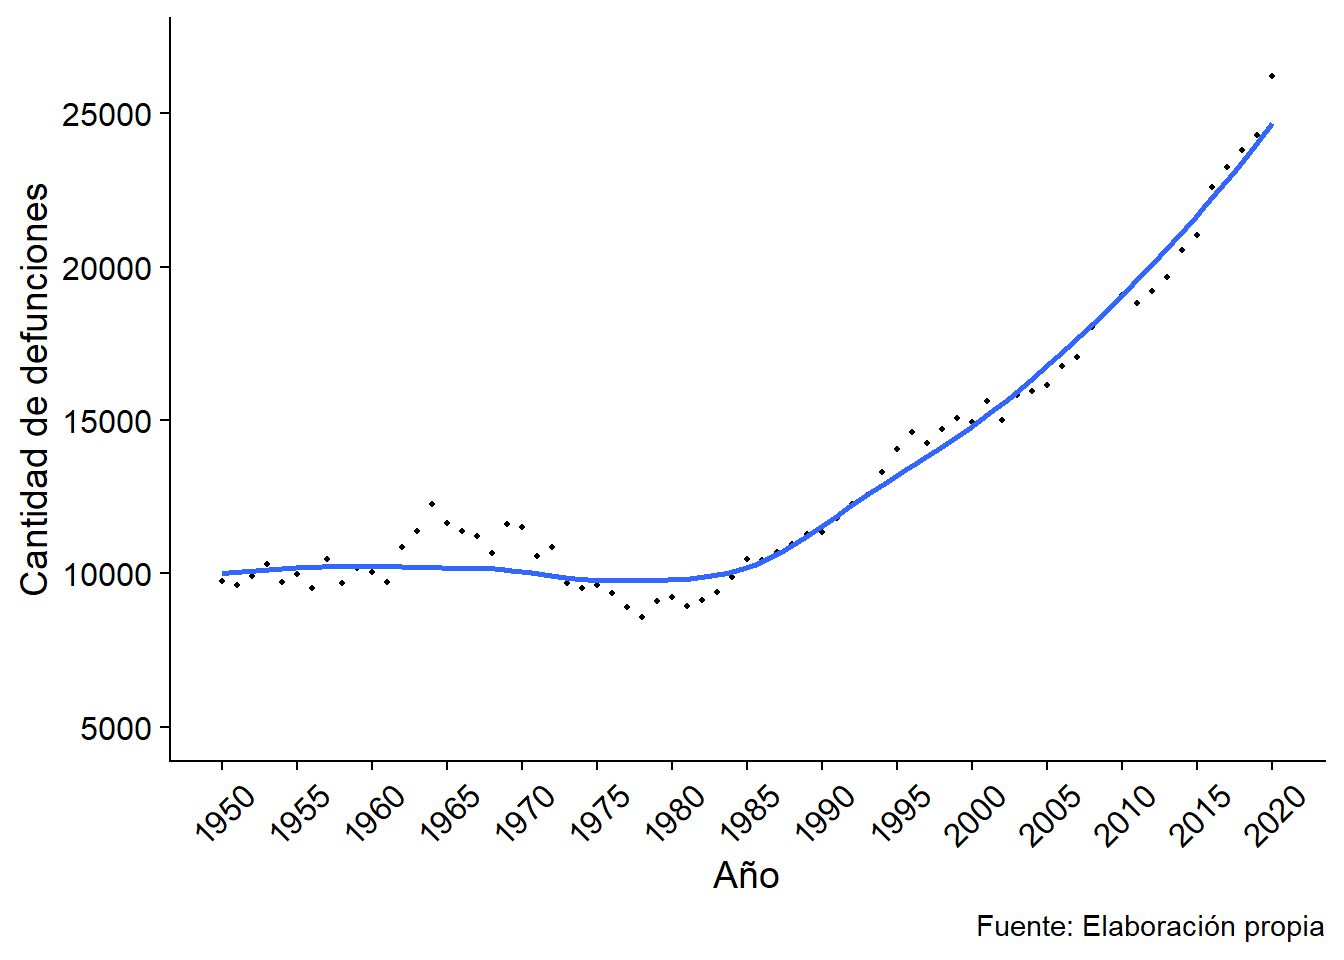
\includegraphics{./Bit3_files/figure-pdf/fig-defunciones_ano-1.pdf}

}

\caption{\label{fig-defunciones_ano}Cantidad de defunciones por año para
el periodo 1950-2020}

\end{figure}

\begin{figure}[H]

{\centering 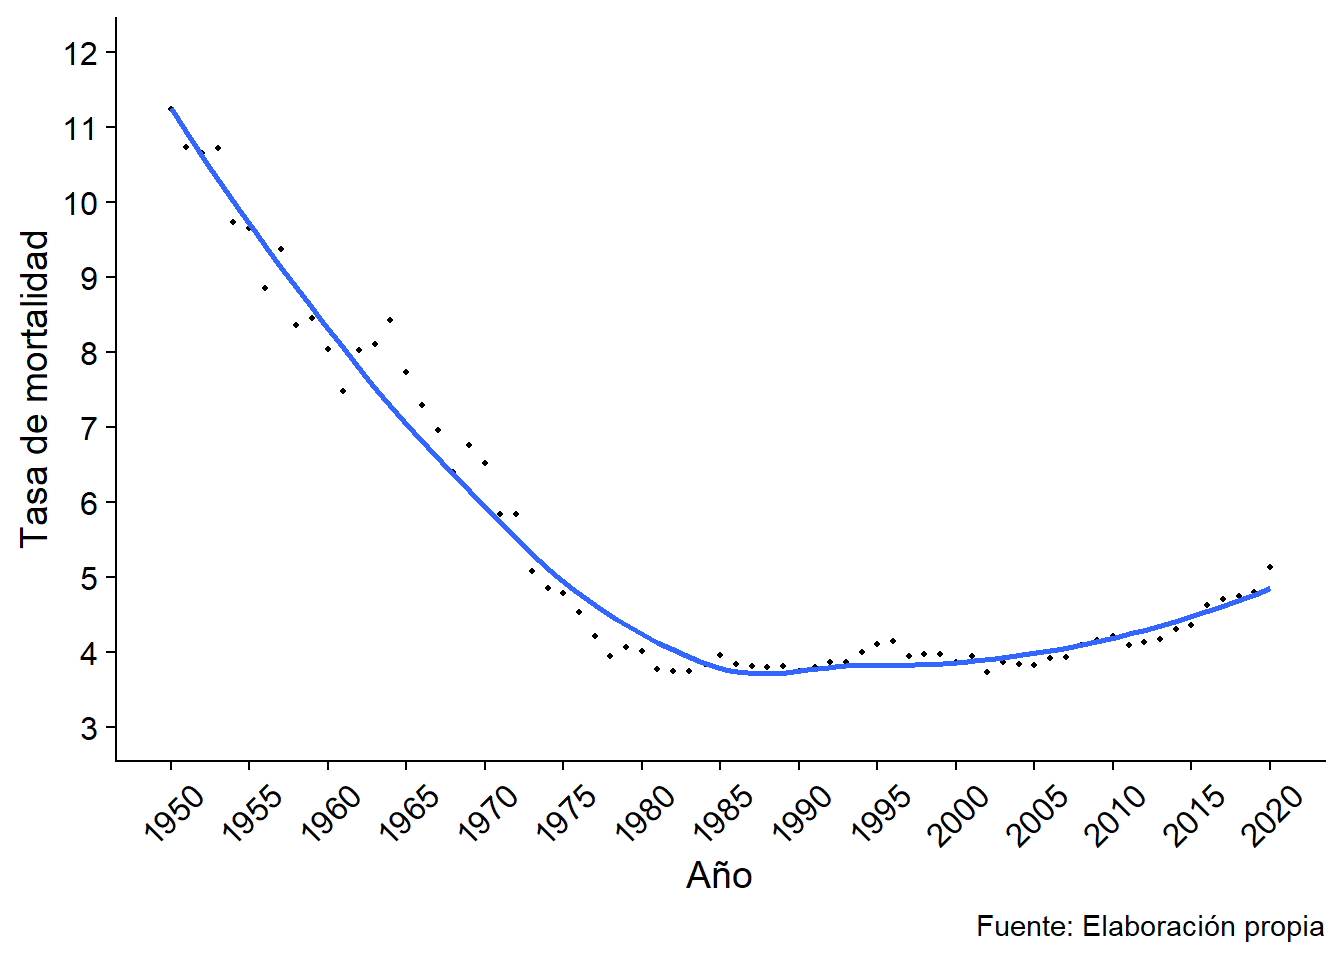
\includegraphics{./Bit3_files/figure-pdf/fig-tasa_mort_ano-1.pdf}

}

\caption{\label{fig-tasa_mort_ano}Tasa de mortalidad por año para el
periodo 1950-2020}

\end{figure}

Este mismo comportamiento se puede observar en la tasa de mortalidad en
la Figura~\ref{fig-tasa_mort_ano} aunque de una forma mucho menos
pronunciada, además, se puede apreciar que para el periodo 1950-1980
esta tasa decreció considerablemente.

\begin{figure}[H]

{\centering 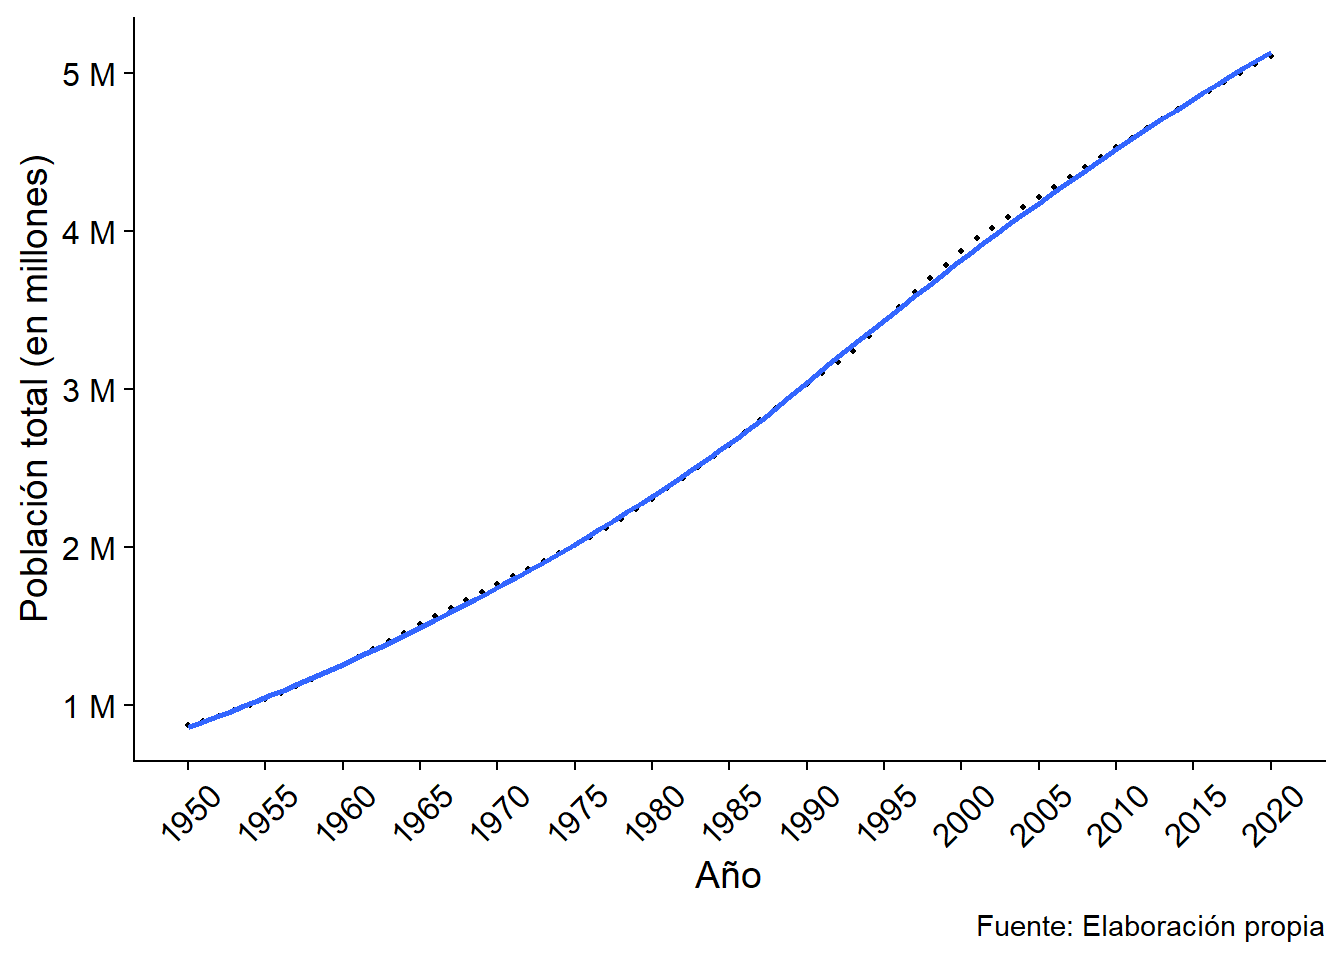
\includegraphics{./Bit3_files/figure-pdf/fig-poblaciones_ano-1.pdf}

}

\caption{\label{fig-poblaciones_ano}Población total por año para el
periodo 1950-2020}

\end{figure}

Por su parte, en la Figura~\ref{fig-poblaciones_ano} se identifica una
clara tendencia creciente de la población durante todo el periodo
considerado.

Asimismo, de la Figura~\ref{fig-nacimientos_ano} se observa que la
cantidad de nacimientos tuvo una tendencia creciente desde el inicio del
periodo hasta cerca de 1990, en que empieza a descender hasta el último
año considerado.

\begin{figure}[H]

{\centering 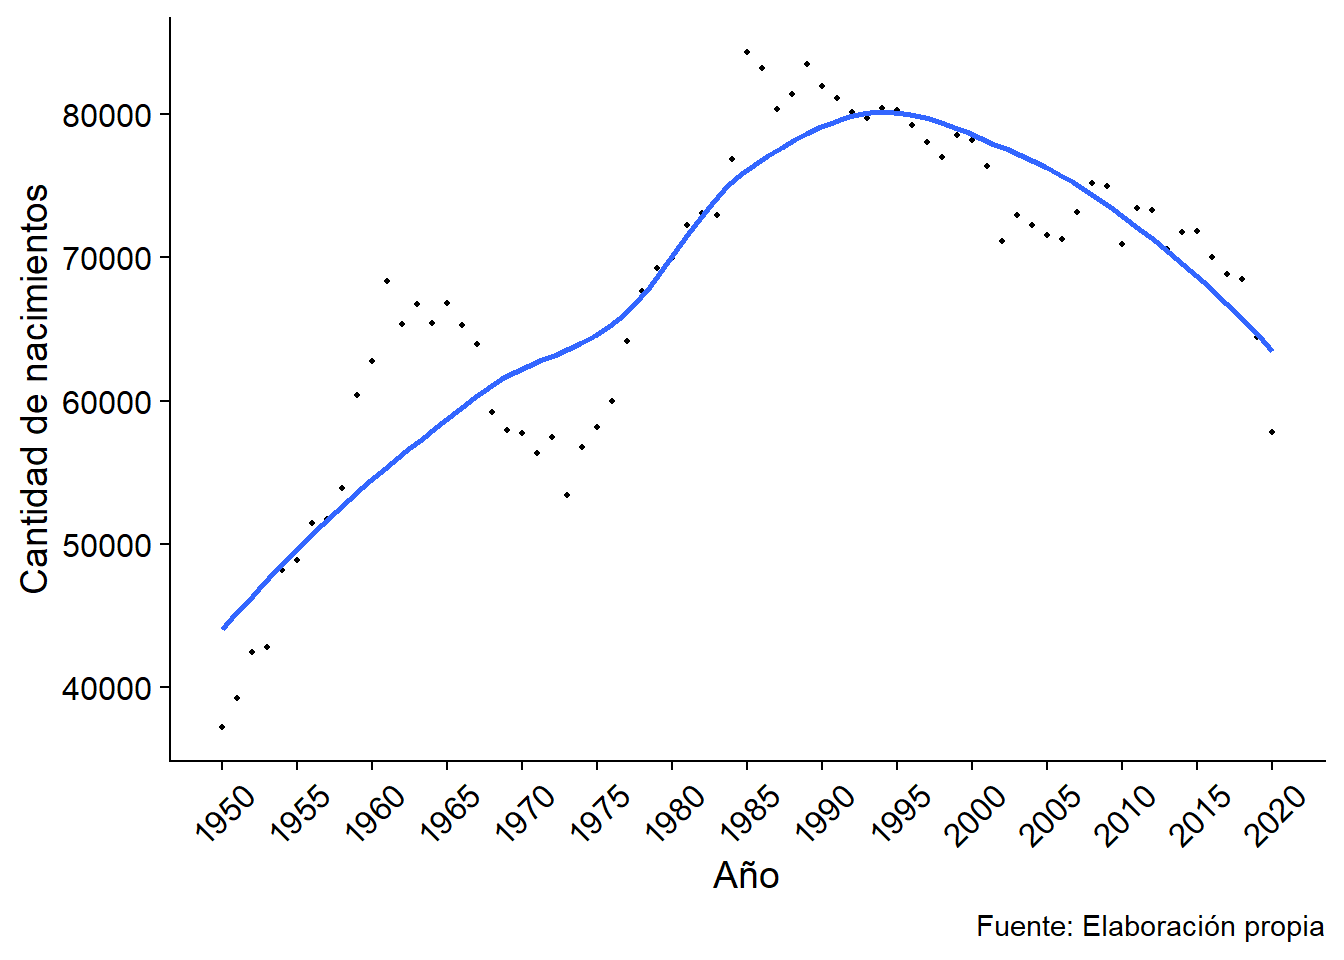
\includegraphics{./Bit3_files/figure-pdf/fig-nacimientos_ano-1.pdf}

}

\caption{\label{fig-nacimientos_ano}Cantidad de nacimientos por año para
el periodo 1950-2020}

\end{figure}

En la Figura~\ref{fig-def_inf_neonat_fet_ano} se comparan las
defunciones infantiles, neonatales y fetales. Cabe añadir que la
distancia verticar entre las defunciones infantiles y las neonatales
resulta en las llamadas defunciones posneonatales, es decir, las que
ocurren a partir de los 29 días de edad y hasta un año. Se advierte que
a mediados de los años sesenta la cantidad de defunciones infantiles
aparenta tener una tendencia decreciente. Al respecto, Rosero Bixby
afirma que la caída más dramática en los años setenta ``se logra gracias
a los programas de atención primaria de la salud, ayudados por una
extraordinaria reducción de la natalidad que permite un mejor desarrollo
intrauterino, mejor cuidado del niño y reduce el riesgo de contagio''
(2004). El mismo autor menciona que ``el riesgo de morir de los menores
de un año ha disminuido en forma poco menos que espectacular entre
1970-78, pues ha sido reducido a la tercera parte (de 62 a 22 muertes
por cada mil nacimientos) en un lapso de apenas 8 años'' (Rosero-Bixby
2016). Por su parte, la cantidad de defunciones neonatales superó a las
fetales desde mediados de los años cincuenta y hasta mediados de los
años ochenta, donde se pierde un poco la noción de cuál suele ser mayor.

\begin{figure}[H]

{\centering 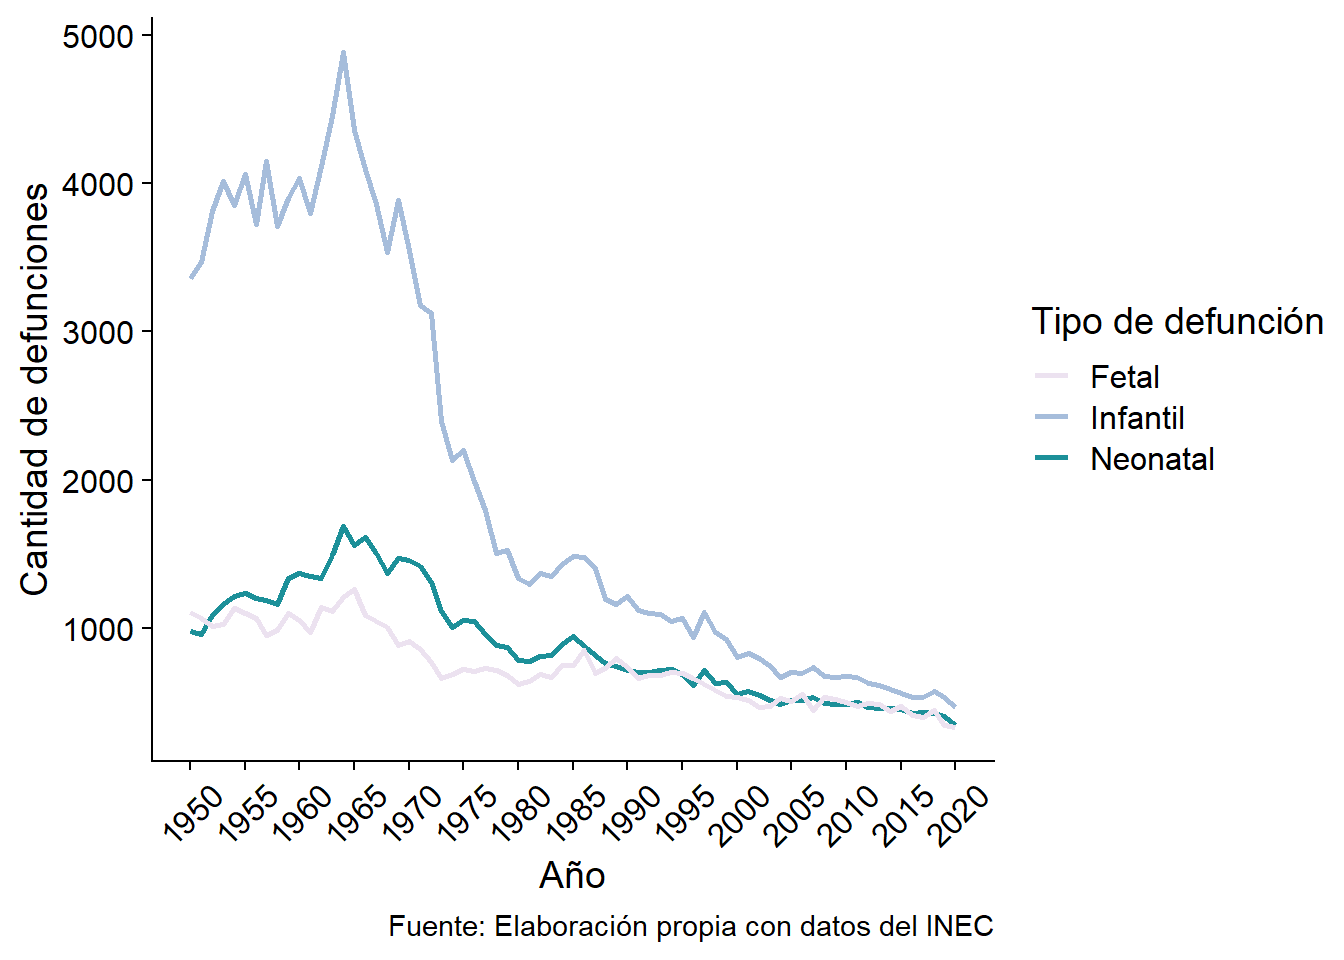
\includegraphics{./Bit3_files/figure-pdf/fig-def_inf_neonat_fet_ano-1.pdf}

}

\caption{\label{fig-def_inf_neonat_fet_ano}Defunciones infantiles,
neonatales y fetales por año}

\end{figure}

Para estudiar la asociación entre la tasa de defunciones neonatales y la
de defunciones fetales, se crea una variable categórica indicadora de si
la primera es mayor a la segunda. Dado que ambas tasas se calculan
respecto al mismo denominador (la cantidad de nacimientos), esta
variable equivale a hacer los mismo con la cantidad de defunciones
respectiva. En la Figura~\ref{fig-indicadora_neonat_fet} se muestra la
distribución de esta variable y se ve que en 15 de los 71 años
considerados la tasa de mortalidad fetal fue mayor, donde de la
Figura~\ref{fig-def_inf_neonat_fet_ano} se sabe que esto sucedió
mayoritariamente entre 1985 y 2020. En consecuencia, en 56 años fue
mayor la tasa de mortalidad neonatal, lo cuál sucede sobre todo en los
primeros 35 años a partir de 1950. Entonces, en los 71 años de estudio,
78.87\% de las ocasiones fue mayor la tasa de mortalidad neonatal,
contra un 21.13\% de la fetal.

\begin{figure}[H]

{\centering 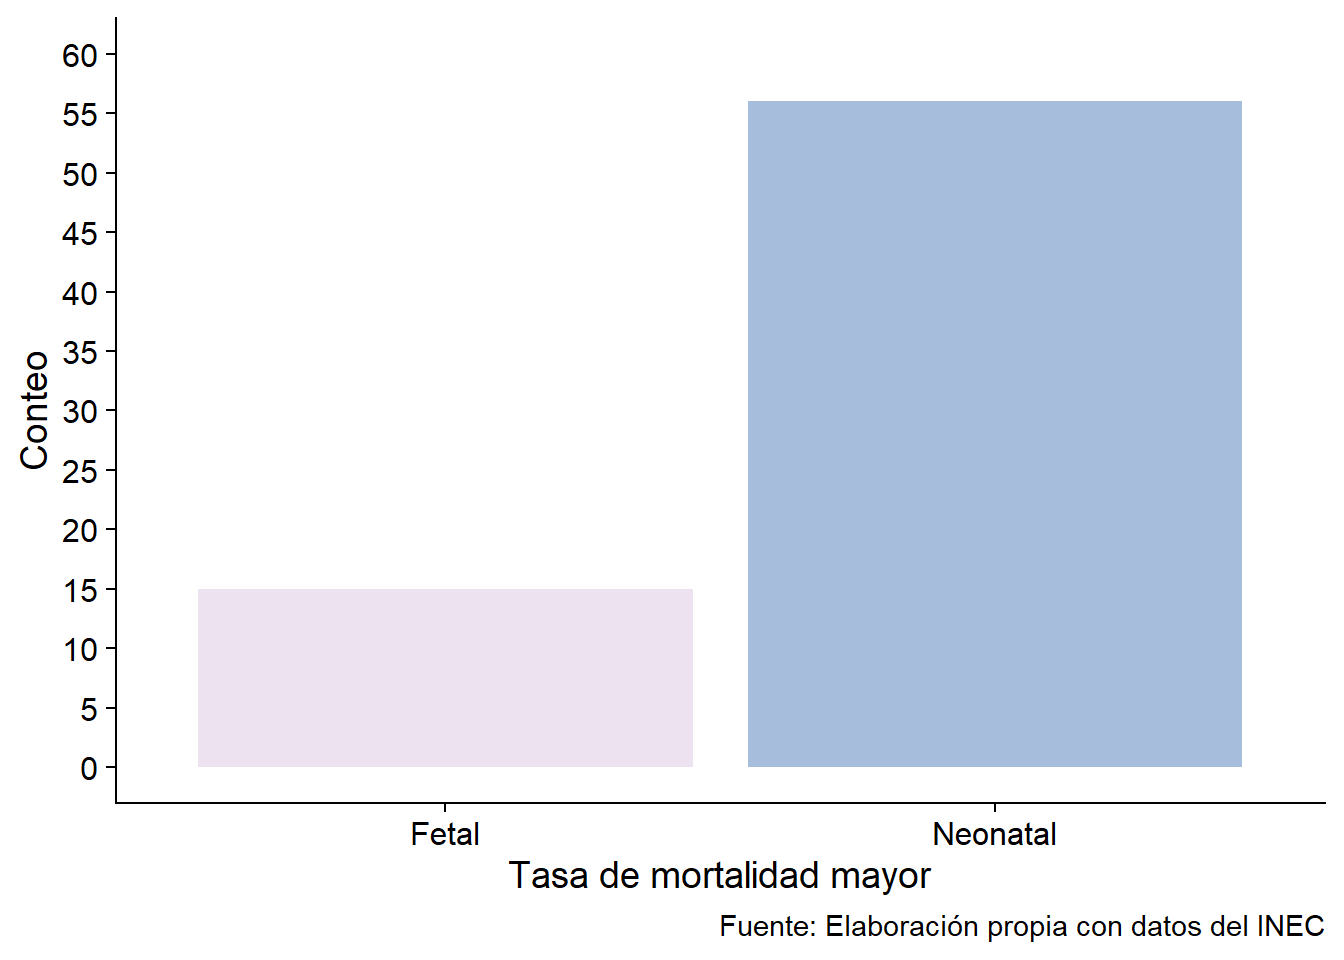
\includegraphics{./Bit3_files/figure-pdf/fig-indicadora_neonat_fet-1.pdf}

}

\caption{\label{fig-indicadora_neonat_fet}Distribución variable
indicadora de la mayor tasa entre las de mortalidad fetal y la neonatal}

\end{figure}

Debido a que, por razones de escala, la cantidad de defunciones,
nacimientos y población total resultan difíciles de comparar
gráficamente, una alternativa se muestra en la
Figura~\ref{fig-tasa_crec_nat_ano}, donde se muestran las tasas de
crecimiento, mortalidad y natalidad por año. Se identifica la gran
similitud en el comportamiento de las tasas de crecimiento y natalidad,
lo cuál no es ninguna sorpresa pues la segunda es una componente aditiva
de la primera. Ahora bien, este gráfico permite apreciar que desde
mediados del siglo XX y hasta cerca de 1980, tanto la tasa de
crecimiento como la de mortalidad aparentan haber tenido una tendencia a
la baja, lo cuál se rompe cerca de dicho año y la tasa de mortalidad
empieza a empinarse ligeramente, mientras que la de crecimiento continúa
en su tenencia con su tendencia decreciente. Nuevamente, se ve que el
año 1980 parece haber un cambio en el comportamiento demográfico del
país.

\begin{figure}[H]

{\centering 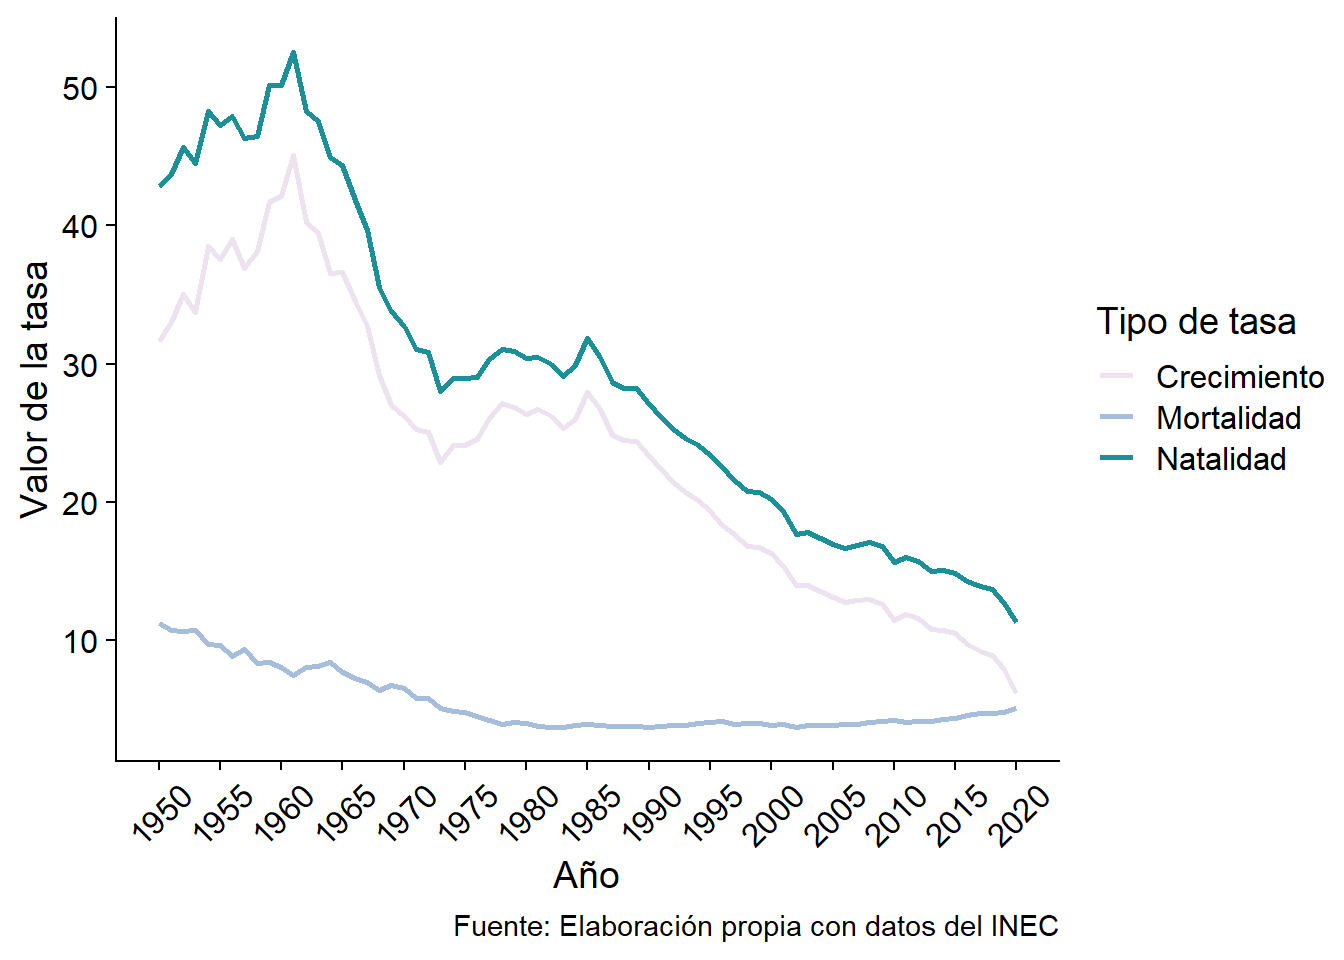
\includegraphics{./Bit3_files/figure-pdf/fig-tasa_crec_nat_ano-1.pdf}

}

\caption{\label{fig-tasa_crec_nat_ano}Tasas de crecimiento, mortalidad y
natalidad por año}

\end{figure}

Para analizar la asociación de la tasa de mortalidad con la de
crecimiento, se crea una variable categórica que indica si entre
periodos consecutivos hubo coincidencia en la monotonía de ambas tasas,
esto es, la variable es verdadera si ambas decrecieron o subieron, y es
falsa si esto no se cumplió. En las figuras
Figura~\ref{fig-hist-coinc-mort-crec} se muestra el histograma de esta
variable, donde se ve que fue más común la no coincidencia en el
comportamiento de las tasas entre periodos consecutivos.

\begin{figure}[H]

{\centering 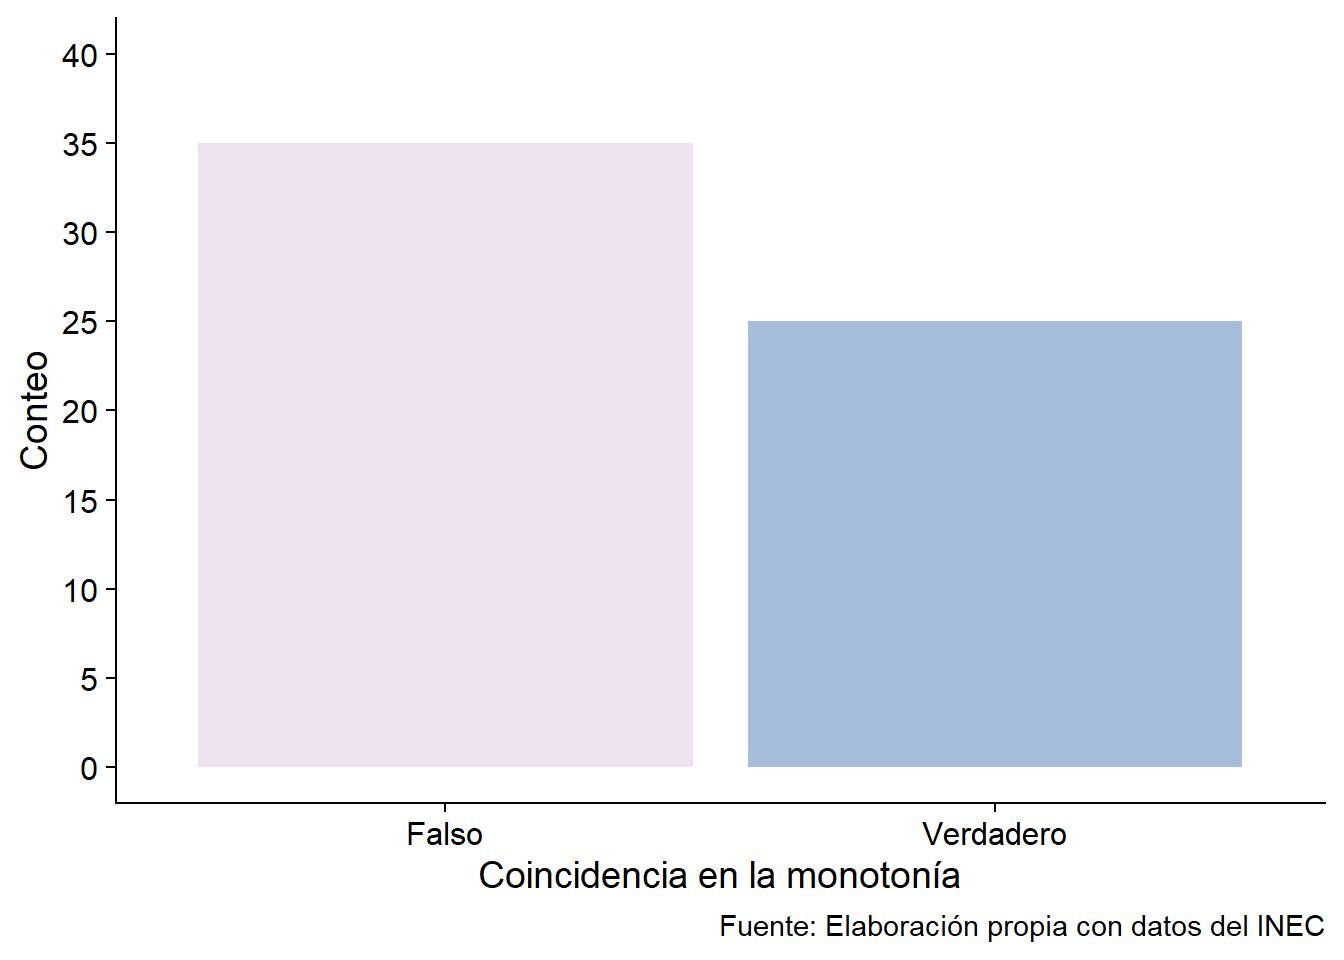
\includegraphics{./Bit3_files/figure-pdf/fig-hist-coinc-mort-crec-1.pdf}

}

\caption{\label{fig-hist-coinc-mort-crec}Histograma de la coincidencia
en la monotonía de la tasa de mortalidad y la de crecimiento}

\end{figure}

En la Figura~\ref{fig-dist-ano-mort-crec} se muestra la distribución de
los años según la coincidencia en la monotonía de la tasa de mortalidad
y la de crecimiento y se ve que esta fue relativamente uniforme. Hacia
2016, se afirmaba que ``la actual tasa de mortalidad general de Costa
Rica (4 muertes anuales por cada mil habitantes) es una de las más bajas
del mundo, inferior incluso a la de los superdesarrollados países de la
Europa Noroccidental (11 por mil) {[}\ldots{]} esta situación tan
favorable se debe, en parte, a una estructura por edades muy particular
de la población costarricense, caracterizada por una alta concentración
en las edades donde la mortalidad es más baja (adultos jóvenes)''
(Rosero-Bixby 2016).

\begin{figure}[H]

{\centering 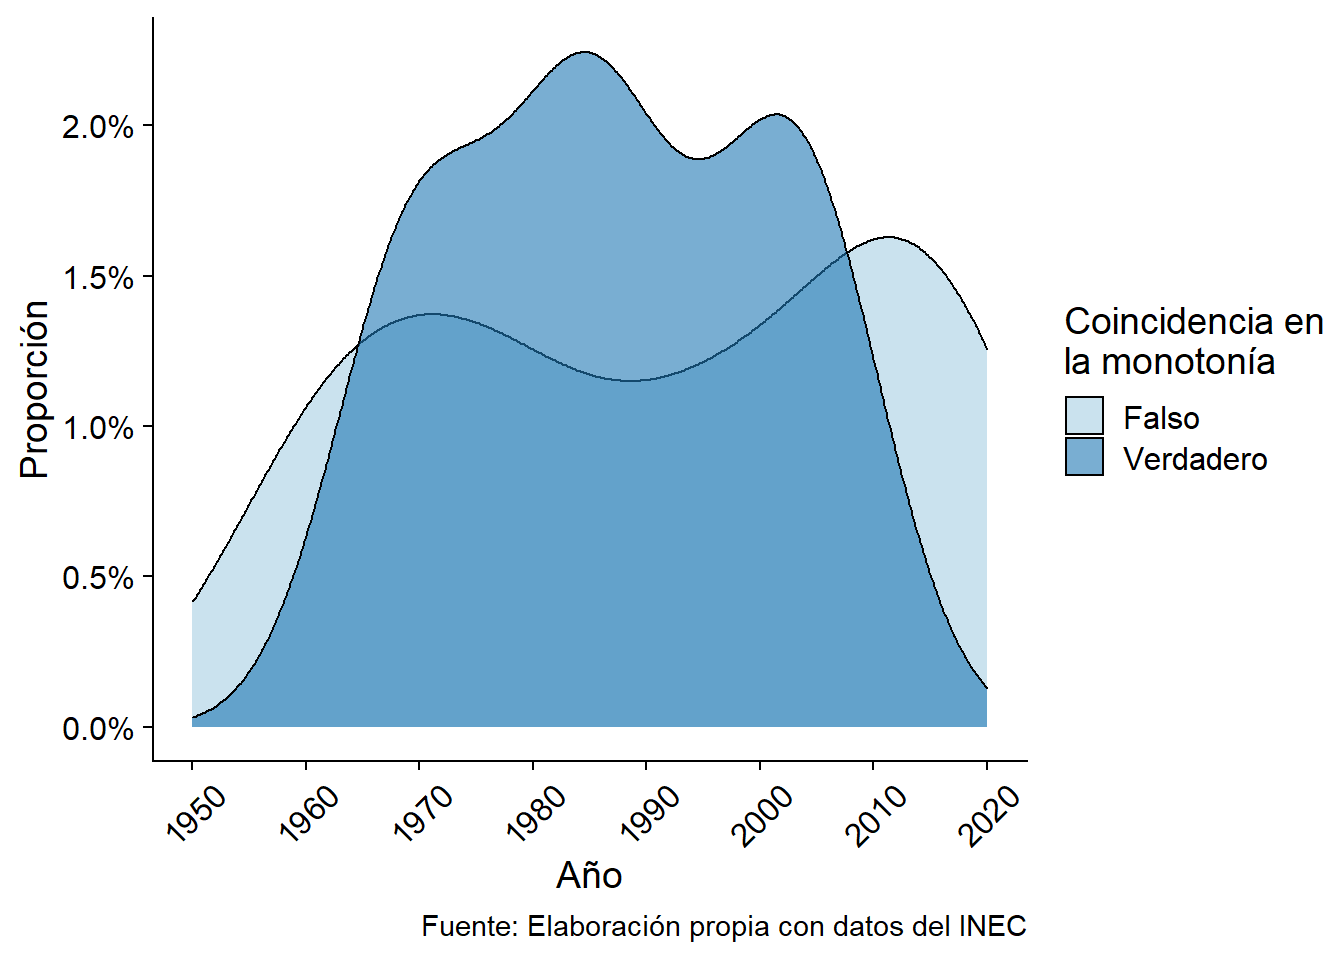
\includegraphics{./Bit3_files/figure-pdf/fig-dist-ano-mort-crec-1.pdf}

}

\caption{\label{fig-dist-ano-mort-crec}Distribución de los años según la
coincidencia en la monotonía de la tasa de mortalidad y la de
crecimiento}

\end{figure}

Se realiza el mismo ejercicio con la población total y las defunciones
totales, lo que resulta en el histograma en la
Figura~\ref{fig-hist-coinc-pob-def} y la distribución de los años en la
Figura~\ref{fig-dist-ano-pob-def}.

\begin{figure}[H]

{\centering 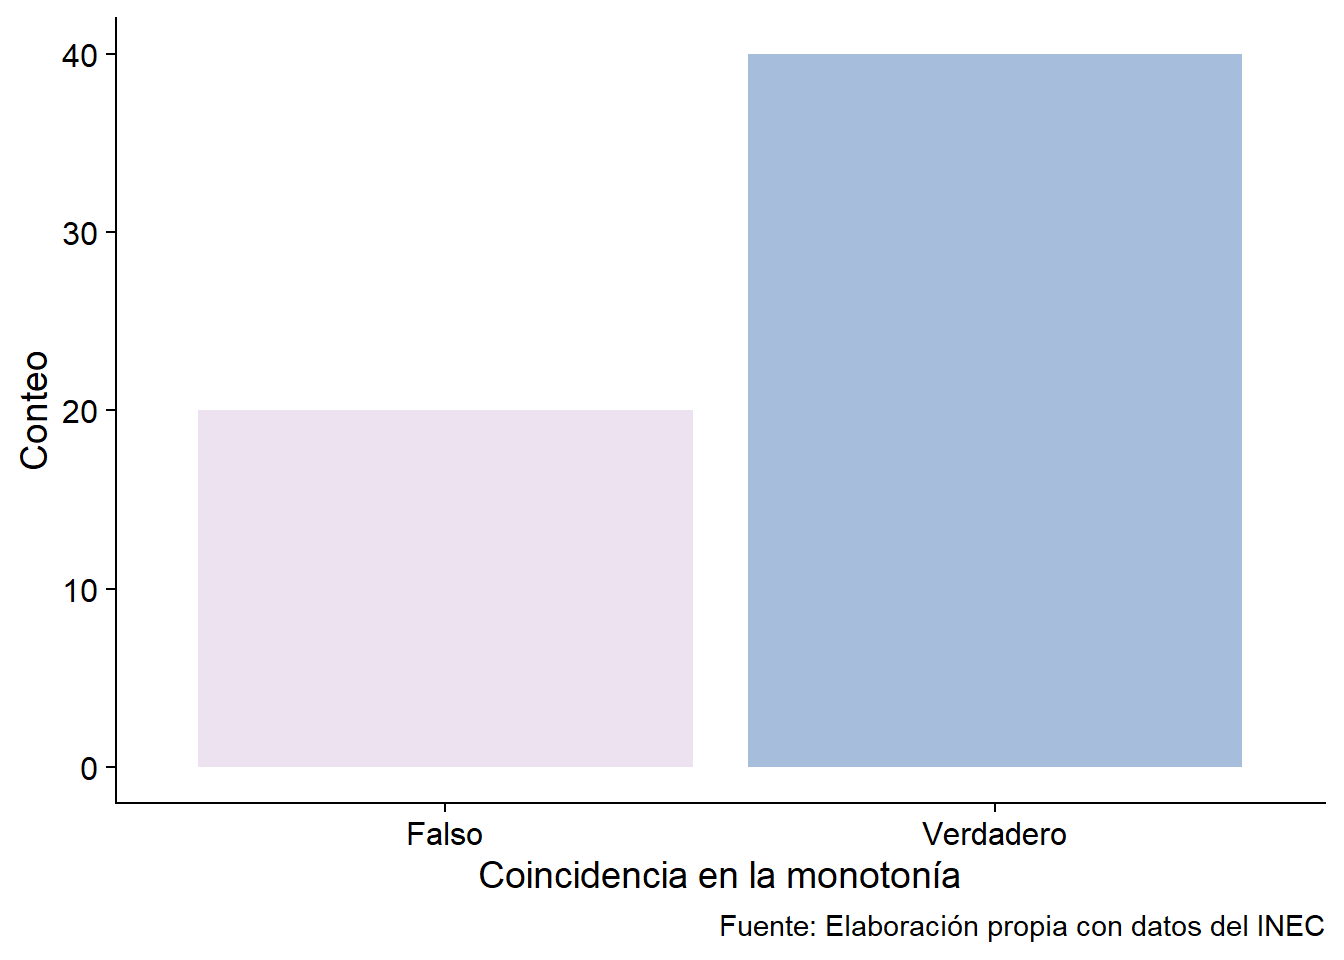
\includegraphics{./Bit3_files/figure-pdf/fig-hist-coinc-pob-def-1.pdf}

}

\caption{\label{fig-hist-coinc-pob-def}Histograma de la coincidencia en
la monotonía de la población total y las defunciones totales}

\end{figure}

De la primera se ve que fue más común la coincidencia en este caso, y de
la segunda que es relativamente marcado que la coincidencia fue falsa de
mediados de los años ochenta para atrás, y fue más común que la
coincidencia se diera desde cerca de 1980. Nuevamente, se haya evidencia
descriptiva de que en la década de los ochenta hay algún tipo de cambio,
lo que debe tenerse en cuenta en la sección metodológica, quizás
restringiendo el periodo de estudio.

\begin{figure}[H]

{\centering 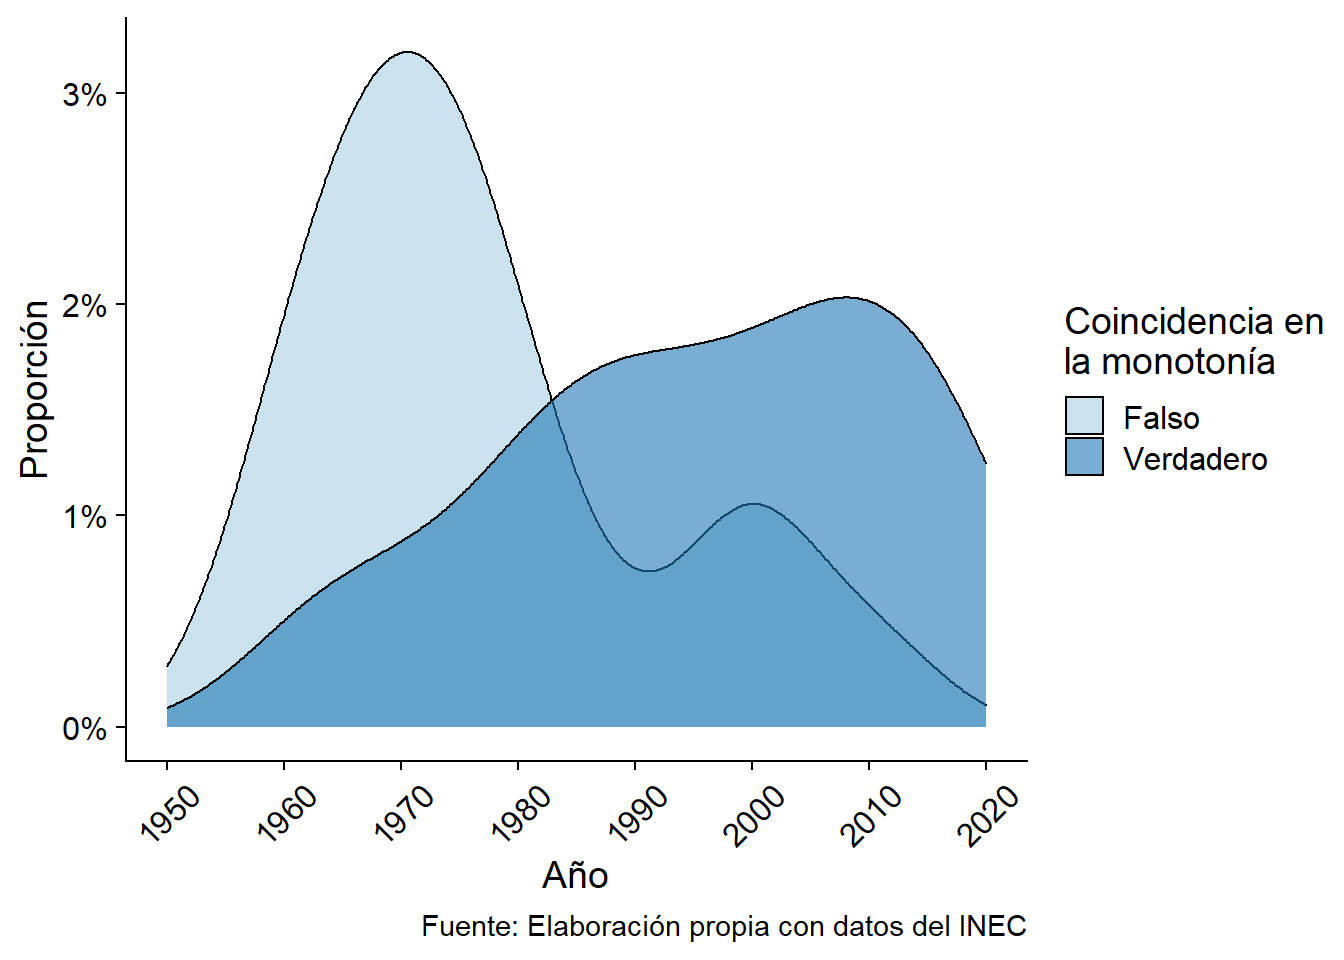
\includegraphics{./Bit3_files/figure-pdf/fig-dist-ano-pob-def-1.pdf}

}

\caption{\label{fig-dist-ano-pob-def}Distribución de los años según la
coincidencia en la monotonía de la población total y la cantidad de
defunciones}

\end{figure}

Se vuelve a proceder de la misma manera, esta vez con las defunciones
infantiles y las defunciones totales, lo que resulta en el histograma en
la Figura~\ref{fig-hist-coinc-infant-def} y la distribución de los años
en la Figura~\ref{fig-dist-ano-infant-def}.

\begin{figure}[H]

{\centering 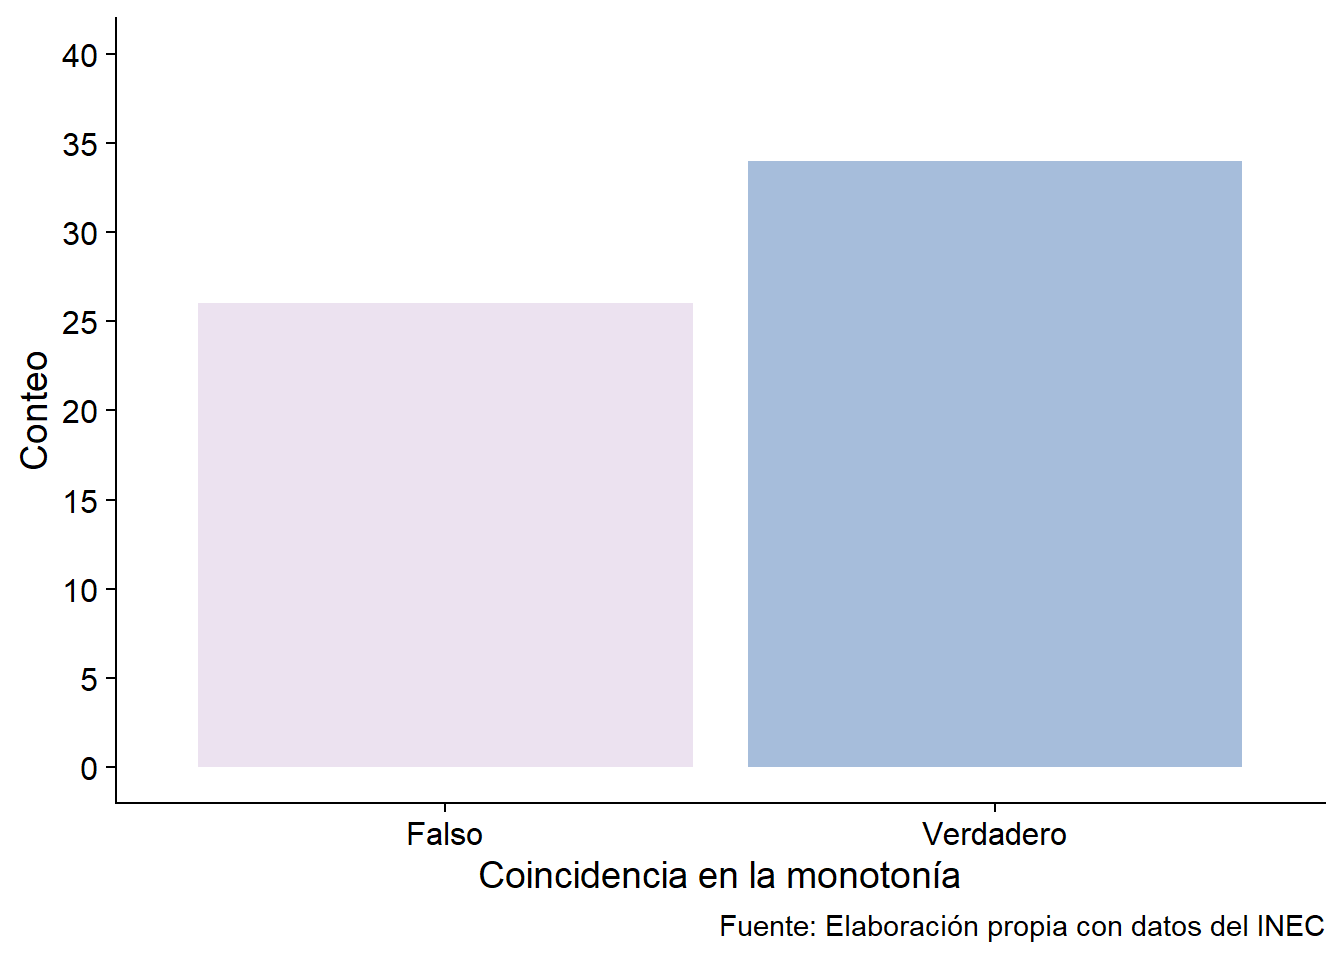
\includegraphics{./Bit3_files/figure-pdf/fig-hist-coinc-infant-def-1.pdf}

}

\caption{\label{fig-hist-coinc-infant-def}Histograma de la coincidencia
en la monotonía de las defunciones infantiles y las defunciones totales}

\end{figure}

En este caso, los conteos están más parejos pero ocurrió más que sí se
diera la coincidencia.

\begin{figure}[H]

{\centering 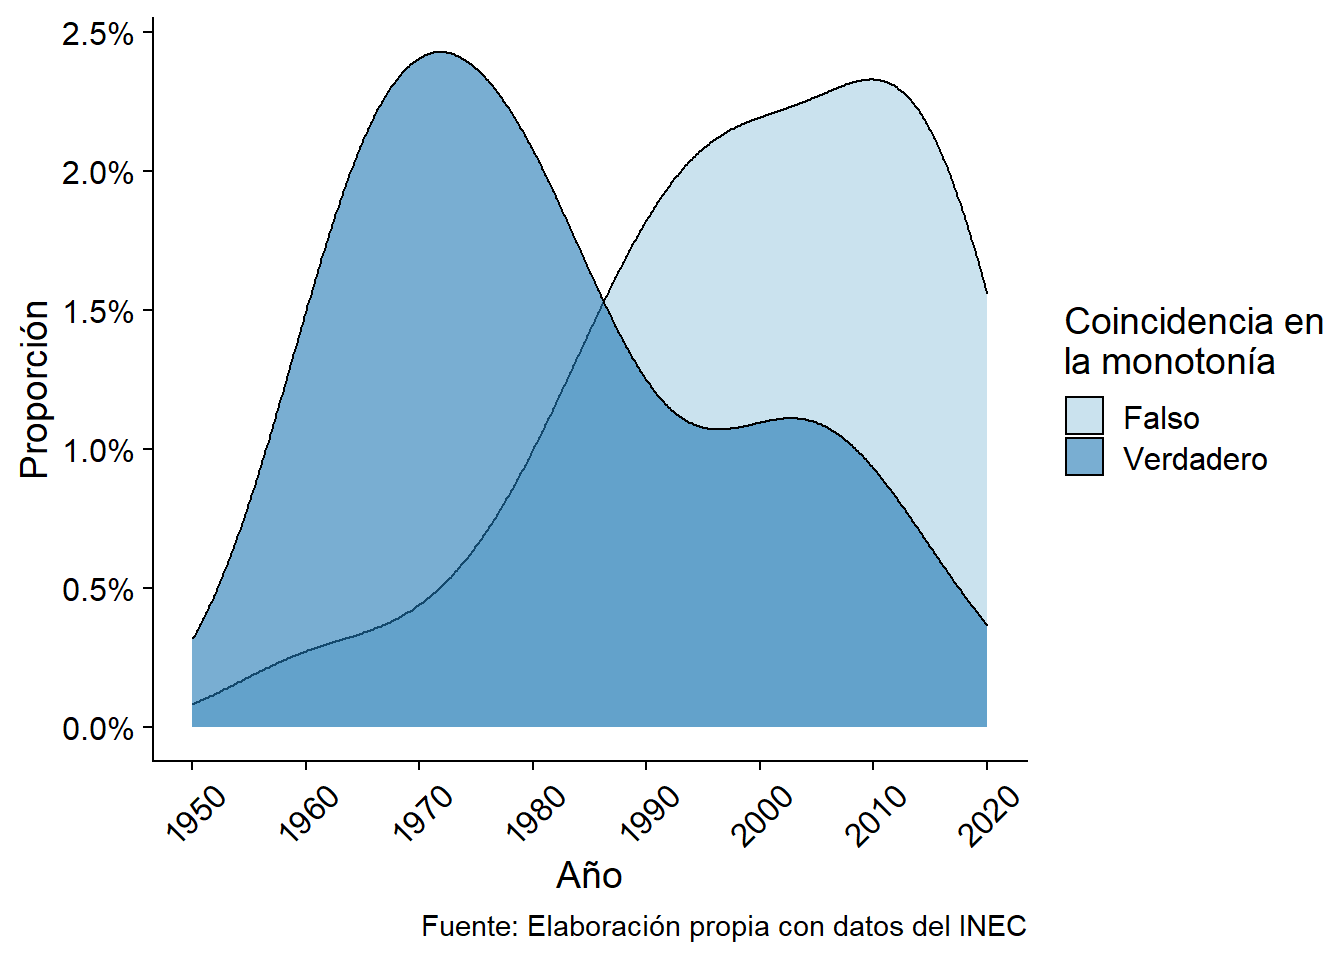
\includegraphics{./Bit3_files/figure-pdf/fig-dist-ano-infant-def-1.pdf}

}

\caption{\label{fig-dist-ano-infant-def}Distribución de los años según
la coincidencia en la monotonía de las defunciones infantiles y la
cantidad de defunciones}

\end{figure}

Además, de las distribuciones se aprecia que la discordancia se dio
cerca de 1980 hasta el final, mientras que la coincidencia ocurrió sobre
todo en años anteriores a 1990. De nuevo, 1980 parece ser un punto de
corte pertinente pues aparenta marcar un cambio en el comportamiento de
las defunciones totales.

\hypertarget{descripciuxf3n-del-modelo-o-metodologuxeda}{%
\section{Descripción del modelo o
metodología}\label{descripciuxf3n-del-modelo-o-metodologuxeda}}

Con la finalidad de realizar un pronóstico de la serie de defunciones
totales anuales de Costa Rica, se desea implementar el modelo
estadístico que mejor se ajuste a los datos.

Para nuestro estudio en cuestión, se ha optado por realizar una
implementación de Modelos de Espacio-Estado.Particularmente, Modelos
Dinámicos Lineales (DLM).

Tal como lo establece Petris, Petrone, y Patrizia (2007), estos últimos
son una clase de Modelos de Espacio-Estado también llamados Modelos de
Espacio-Estado Lineales Gaussianos. Estos modelos son especificados
mediante dos ecuaciones, para \(t \geq 1\) se tiene:

\[ Y_{t}= F_{t} \theta_{t} + v_{t} , \]
\[  \theta_{t}= G_{t} \theta_{t-1} + w_{t}   \]

Donde la primer ecuación es llamada ecuación de observación, y la
segunda ecuación estado o ecuación del sistema.

Es importante señalar que \(F_{t}\) y \(G_{t}\) son matrices y
\((v_{t})\) , \((w_{t})\) son secuencias de ruidos blancos
independientes tales que:

\[ v_{t} \sim \mathcal{N}_{m}(0,V_{t}) , \]
\[  w_{t} \sim \mathcal{N}_{p}(0,W_{t})  \]

Los DLM poseen dos supuestos, la linealidad y el supuesto de
distribuciones Gaussianas. Petris, Petrone, y Patrizia (2007) señala que
este último supuesto puede ser justificado mediante argumentos del
teorema del límite central.

La estimación y pronóstico se pueden resolver calculando las
distribuciones condicionales de las cantidades de interés, dada la
información disponible. Para estimar el vector de estados es necesario
computar la densidad condicional \(p(\theta_{t} |y_{1}, .., y_{t})\). En
particular, nos interesa el problema de filtrado (cuando \(s=t\)), donde
los datos se supone que llegan secuencialmente en el tiempo.

En general, el problema de pronóstico de \(k\)-pasos hacia adelante
consiste en estimar la evolución del sistema \(\theta_{t+k}\) para
\(k \geq 1\) y realizar un pronóstico de \(k\)-pasos para \(Y_{t+k}\).

Según Petris, Petrone, y Patrizia (2007) en los DLM, el filtro de Kalman
proporciona las fórmulas para actualizar nuestra inferencia actual sobre
el vector de estado conforme se disponga de nuevos datos.

Para un DLM, si se cumple que:

\[ \theta_{t} | \mathcal{D}_{t} \sim \mathcal{N}(m_{t}, C_{t}) , t \geq 1 \]

Se tiene que:

La densidad de predicción de estado de k-pasos con \(k \geq 1\) hacia
adelante de \(\theta_{t+k}\) dada la información pasada \(D_{t}\), es
Gaussiana con media y varianza condicional dadas respectivamente por:

\[  a_{t+k} = G_{t+k}m_{t} \]
\[ R_{t+k}= G_{t+k}C_{t+k}G^{'}_{t+k} + W_{t+k} \]

La densidad de predicción de \(k\)-pasos con \(k \geq 1\) hacia adelante
de \(Y_{t+k}\) dada la información pasada \(D_{t}\), es Gaussiana con
media y varianza condicional dadas respectivamente por:

\[  f_{t+k} = F_{t+k}a_{t+k} \]
\[ Q_{t+k}= F_{t+k}R_{t+k}F^{'}_{t+k} + V_{t+k} \]

La densidad de filtrado de \(\theta_{t+k}\) con \(k \geq 1\) dada la
información pasada \(D_{t+k}\), es Gaussiana con media y varianza
condicional dadas respectivamente por:

\[  m_{t+k} = a_{t+k} + R_{t+k}F^{'}_{t+k}Q^{-1}_{t+k}e_{t+k} \]
\[ C_{t+k}=R_{t+k} - R_{t+k}F^{'}_{t+k}Q^{-1}_{t+k}F_{t+k}R_{t+k}  \]

\hypertarget{propuesta-y-justificaciuxf3n-modelos-dlm}{%
\section{Propuesta y justificación modelos
DLM}\label{propuesta-y-justificaciuxf3n-modelos-dlm}}

Como se mencionó en Figura~\ref{fig-defunciones_ano} , la cantidad de
defunciones totales siguen una cierta tendencia lineal creciente, en
particular para años posteriores a 1980.

Debido a que esta es nuestra variable de interés para realizar un
pronóstico, es propicio para nuestro estudio en cuestión la
implementación de un modelo con supuesto de linealidad, como se mencionó
justamente los DLM siguen este supuesto.

Para llevar a cabo los pronósticos se proponen por tanto tres métodos
estadísticos pertenecientes a los DLM, estos son: modelo DLM polinomial
de primer orden, modelo DLM polinomial de segundo orden y el modelo
ARIMA.

Se propone un modelo DLM de primer orden ya que como establece Mary
(2006) los DLM de primer orden son algoritmos recomendados al lidiar con
datos anuales debido a que las series de tiempo es corta y no presentan
patrones estacionales.Dado que nuestros datos son anuales, este modelo
se presenta como un posible candidato.

Por su parte Mary (2006), señala que los DLM de segundo orden son útiles
para describir tendencias. Dada la tendencia observada de la serie de
defunciones totales sugiere por tanto realizar un modelo polinomial de
segundo orden.

\hypertarget{primera-implementaciuxf3n}{%
\section{Primera implementación}\label{primera-implementaciuxf3n}}

Como una primer implementación se utilizará un modelo ARIMA. Tal como lo
menciona Petris, Petrone, y Patrizia (2007) un modelo ARIMA puede ser
considerado un DLM, esto ya que es posible representar todo modelo ARIMA
(ya sea univariado o mulltivariado) como un DLM.

La escogencia de este modelo al ser un DLM, sigue la misma línea de
justificación antes mencionado sobre la elección de modelos DLM para
nuestro estudio, siendo este un caso particular de estos.

Sin embargo, es importante mencionar que la escogencia de este modelo
como primera implementación también se basa en su simplicidad, y en que
dada la bibliografía consultada, se observa que en múltiples
investigaciones con temáticas relacionadas a nuestro estudio como el de
Adekanmbi, Ayoola, y Idowu (2014) y el estudio por Ordorica (2004) , se
implementa este tipo de modelo.

No obstante, según Petris, Petrone, y Patrizia (2007) estos modelos
proporcionan un enfoque de caja negra para el análisis de datos,
ofreciendo la posibilidad de predecir observaciones futuras, pero con
una interpretabilidad muy limitada del modelo ajustado.

Por lo que para bitácoras posteriores se describirán en detalle e
implementaran dos modelos de mayor complejidad pero con una mejor
interpretabilidad, como lo son los DLM polinomiales de primer y segundo
orden, antes mencionados.

En cuanto a la implementación del primer intento utilizando ARIMA, como
se quiere hacer una comparación entre los modelos, se usará una base de
entrenamiento y una de prueba para hacer el diagnóstico y cuyos valores
ya son conocido para poder valorar la eficacia de dicho modelo. Se
quiere hacer el pronóstico a dos años, por lo que la base entrenamiento
será los datos entre 1950 y 2018, y se pronosticará las defunciones
totales para el 2019 y 2020.

\begin{Shaded}
\begin{Highlighting}[]
\NormalTok{entrenamiento }\OtherTok{\textless{}{-}}\NormalTok{ base}\SpecialCharTok{$}\NormalTok{defunciones[}\DecValTok{1}\SpecialCharTok{:}\DecValTok{69}\NormalTok{]}
\NormalTok{serie }\OtherTok{\textless{}{-}} \FunctionTok{ts}\NormalTok{( entrenamiento, }\AttributeTok{start=}\FunctionTok{c}\NormalTok{(}\DecValTok{1950}\NormalTok{,}\DecValTok{1}\NormalTok{), }\AttributeTok{frequency=}\DecValTok{1}\NormalTok{)}
\end{Highlighting}
\end{Shaded}

Primero, se grafica la serie de tiempo de defunciones totales. Para
emplear el modelo se requiere estacionareidad.

\begin{figure}[H]

{\centering \includegraphics{./Bit3_files/figure-pdf/fig-serieDefunciones-1.pdf}

}

\caption{\label{fig-serieDefunciones}Serie de tiempo de defunciones
totales}

\end{figure}

\begin{verbatim}
     [,1]  [,2]  [,3] [,4]  [,5]  [,6]  [,7]  [,8]  [,9] [,10] [,11] [,12]
ACF  0.93  0.86  0.80 0.74  0.69  0.64  0.59  0.54  0.49  0.43  0.38  0.34
PACF 0.93 -0.02 -0.04 0.06 -0.02 -0.01 -0.02 -0.03 -0.08  0.00 -0.03  0.01
     [,13] [,14] [,15] [,16] [,17] [,18] [,19]
ACF    0.3  0.26  0.23  0.20  0.17  0.13   0.1
PACF   0.0  0.00  0.02 -0.05  0.02 -0.09   0.0
\end{verbatim}

\begin{figure}[H]

{\centering \includegraphics{./Bit3_files/figure-pdf/fig-ACFDefunciones-1.pdf}

}

\caption{\label{fig-ACFDefunciones}ACF y PACF de la serie de defunciones
totales}

\end{figure}

Se observa de la Figura~\ref{fig-serieDefunciones} no estacionareidad
muy clara, además de que la decadencia de las correlaciones no son
suficientemente rápidas. Se lleva a cabo una diferenciación

\begin{figure}[H]

{\centering \includegraphics{./Bit3_files/figure-pdf/fig-serieDefuncionesdif-1.pdf}

}

\caption{\label{fig-serieDefuncionesdif}Serie de tiempo de defunciones
totales con una diferencia}

\end{figure}

\begin{verbatim}
     [,1] [,2] [,3]  [,4] [,5] [,6] [,7]  [,8]  [,9] [,10] [,11] [,12] [,13]
ACF     0 0.29 0.11  0.00 0.28 0.02 0.26 -0.01  0.03  0.18 -0.05  0.07  0.08
PACF    0 0.29 0.12 -0.09 0.23 0.04 0.14 -0.08 -0.07  0.15 -0.03 -0.13  0.11
     [,14] [,15] [,16] [,17] [,18] [,19]
ACF  -0.09  0.11  0.00  0.04 -0.08  0.02
PACF -0.10  0.02  0.08 -0.03 -0.14  0.10
\end{verbatim}

\begin{figure}[H]

{\centering \includegraphics{./Bit3_files/figure-pdf/fig-ACFDefuncionesdif-1.pdf}

}

\caption{\label{fig-ACFDefuncionesdif}ACF y PACF de la serie de
defunciones totales con una diferencia}

\end{figure}

Se observa de la Figura~\ref{fig-serieDefuncionesdif} que aún hay
evidencia de no estacionareidad por lo que se lleva a cabo una segunda
diferenciación

\begin{figure}[H]

{\centering \includegraphics{./Bit3_files/figure-pdf/fig-serieDefuncionesdif2-1.pdf}

}

\caption{\label{fig-serieDefuncionesdif2}Serie de tiempo de defunciones
totales con dos diferencias}

\end{figure}

\begin{verbatim}
      [,1]  [,2]  [,3]  [,4]  [,5]  [,6] [,7]  [,8]  [,9] [,10] [,11] [,12]
ACF  -0.65  0.23 -0.03 -0.20  0.27 -0.24 0.25 -0.15 -0.07  0.19 -0.16  0.05
PACF -0.65 -0.33 -0.09 -0.37 -0.15 -0.22 0.01  0.02 -0.20 -0.04  0.09 -0.13
     [,13] [,14] [,15] [,16] [,17] [,18] [,19]
ACF   0.10 -0.20  0.15 -0.06  0.07 -0.09  0.01
PACF  0.08 -0.06 -0.13 -0.01  0.09 -0.15 -0.12
\end{verbatim}

\begin{figure}[H]

{\centering \includegraphics{./Bit3_files/figure-pdf/fig-ACFDefuncionesdif2-1.pdf}

}

\caption{\label{fig-ACFDefuncionesdif2}ACF y PACF de la serie de
defunciones totales con dos diferencias}

\end{figure}

En la Figura~\ref{fig-serieDefuncionesdif2} se aprecia que con dos
diferencias ya se logra estacionareidad. Además, de la
Figura~\ref{fig-ACFDefuncionesdif2} se nota que tiene una decadencia
gradual en las correlaciones y las autocorrelaciones parciales luego del
primer rezago por lo que implica un modelo ARMA(1,1). Se lleva a cabo la
implementación de este modelo con dos rezagos.

\begin{Shaded}
\begin{Highlighting}[]
\NormalTok{modelo }\OtherTok{\textless{}{-}} \FunctionTok{arima}\NormalTok{(serie, }\AttributeTok{order=}\FunctionTok{c}\NormalTok{(}\DecValTok{1}\NormalTok{, }\DecValTok{2}\NormalTok{, }\DecValTok{1}\NormalTok{))}
\end{Highlighting}
\end{Shaded}

y se presentan algunos diagnósticos.

\begin{figure}[H]

{\centering \includegraphics{./Bit3_files/figure-pdf/fig-diagARIMA-1.pdf}

}

\caption{\label{fig-diagARIMA}Diagnósticos del modelo ARIMA
implementado}

\end{figure}

En la Figura~\ref{fig-diagARIMA} se aprecia que los residuos no parecen
mostrar ningún patrón significante y la varianza aparenta ser constante.
El gráfico de ACF confirma que no existe correlación en los residuos. En
el último gráfico se muestra que bajo la prueba de Ljung-Box en cada
rezago se encuentra evidencia estadística de bondad de ajuste del modelo
seleccionado. Finalmente, con este modelo se lleva a cabo el diagnóstico
a dos años.

\begin{figure}[H]

{\centering \includegraphics{./Bit3_files/figure-pdf/fig-pronARIMA-1.pdf}

}

\caption{\label{fig-pronARIMA}Pronóstico a dos años utilizando el modelo
ARIMA}

\end{figure}

\hypertarget{tbl-proARIMA}{}
\begin{table}
\caption{\label{tbl-proARIMA}Pronóstico e intervalos de confianza del modelo ARIMa }\tabularnewline

\centering
\resizebox{\linewidth}{!}{
\begin{tabular}[t]{l|r|r|r|r|r}
\hline
\textbf{ } & \textbf{Point Forecast} & \textbf{Lo 80} & \textbf{Hi 80} & \textbf{Lo 95} & \textbf{Hi 95}\\
\hline
\cellcolor{gray!6}{2019} & \cellcolor{gray!6}{24474.97} & \cellcolor{gray!6}{23840.77} & \cellcolor{gray!6}{25109.17} & \cellcolor{gray!6}{23505.04} & \cellcolor{gray!6}{25444.90}\\
\hline
2020 & 25125.82 & 24253.67 & 25997.98 & 23791.97 & 26459.67\\
\hline
\end{tabular}}
\end{table}

La Tabla~\ref{tbl-proARIMA} resumen los pronósticos e intervalos de
confianzo utilizando el modelo ARIMA que se pueden comparar con los
valores reales de 24292 para el 2019 y 26209 para el 2020. Es importante
recordar que el 2020 fue anómalo por ser el primer año del COVID-19 en
Costa Rica lo que ocasionó más muertes. Áún así se aprecia que para
ambos años se obtuvieron valores que caen dentro del intervalod de
confianza 95\%. La diferencia entre el pronóstico y el valor real en
valor absoluto es dado por

\begin{verbatim}
[1] 182.9708
\end{verbatim}

\begin{verbatim}
[1] 1083.177
\end{verbatim}

\bookmarksetup{startatroot}

\hypertarget{references}{%
\chapter*{References}\label{references}}
\addcontentsline{toc}{chapter}{References}

\hypertarget{refs}{}
\begin{CSLReferences}{1}{0}
\leavevmode\vadjust pre{\hypertarget{ref-adekambi}{}}%
Adekanmbi, D, F Ayoola, y A Idowu. 2014. {«Demographic Time Series
Modelling of Total Deaths in Nigeria»}. \emph{Population Association of
Southern Africa} 15 (1): 21-48.

\leavevmode\vadjust pre{\hypertarget{ref-brownlee}{}}%
Brownlee, Jason. 2020. \emph{{Introduction to time series forcasting
with Python }}. eBook.

\leavevmode\vadjust pre{\hypertarget{ref-INEC_conceptos}{}}%
{«Indicadores demográficos 2019»}. 2020.

\leavevmode\vadjust pre{\hypertarget{ref-INEC_base}{}}%
INEC. 2021. {«{Estadísticas demográficas. 1950-2020. Principales
Indicadores Demográficos}»}.
\url{\%7Bhttps://www.inec.go.cr/documento/estadisticas-demograficas-1950-2020-principales-indicadores-demograficos\%7D}.

\leavevmode\vadjust pre{\hypertarget{ref-maccio1985diccionario}{}}%
Macció, Guillermo A, Santiago Centro Latinoamericano de Demografia,
et~al. 1985. {«Diccionario demogr{á}fico multilingue»}.

\leavevmode\vadjust pre{\hypertarget{ref-optimalDLM}{}}%
Mary, Kathleen. 2006. {«Determining optimal architecture for dynamic
linear models in time serires applications»}.

\leavevmode\vadjust pre{\hypertarget{ref-ordorika}{}}%
Ordorica, Manuel. 2004. {«Pronóstico de las defunciones por medio de los
modelos autorregresivos integrados de promedios móviles»}.
\emph{249--264} 10 (42): 21-48.

\leavevmode\vadjust pre{\hypertarget{ref-petrisDLM}{}}%
Petris, Giovanni, Petrone Sonia, y Campagnoli Patrizia. 2007.
\emph{Dynamic Linear Models with R}. Springer.

\leavevmode\vadjust pre{\hypertarget{ref-REES2020239}{}}%
Rees, Philip. 2020. {«Demography»}. En \emph{International Encyclopedia
of Human Geography (Second Edition)}, editado por Audrey Kobayashi,
Second Edition, 239-56. Oxford: Elsevier.
https://doi.org/\url{https://doi.org/10.1016/B978-0-08-102295-5.10252-5}.

\leavevmode\vadjust pre{\hypertarget{ref-rosero2004situacion}{}}%
Rosero-Bixby, Luis. 2004. {«Situaci{ó}n demogr{á}fica general de Costa
Rica»}.

\leavevmode\vadjust pre{\hypertarget{ref-rosero2016situacion}{}}%
---------. 2016. {«{La situaci{ó}n demogr{á}fica en Costa Rica}»}.
\emph{{Poblaci{ó}n y Salud en Mesoam{é}rica}} 13 (2): 237-311.

\leavevmode\vadjust pre{\hypertarget{ref-wickham2016r}{}}%
Wickham, Hadley, y Garrett Grolemund. 2016. \emph{R for data science:
import, tidy, transform, visualize, and model data}. " O'Reilly Media,
Inc.".

\leavevmode\vadjust pre{\hypertarget{ref-wilson2021brief}{}}%
Wilson, Tom, y Philip Rees. 2021. {«A brief guide to producing a
national population projection»}. \emph{Australian Population Studies} 5
(1): 77-100.

\end{CSLReferences}



\end{document}
